\subsection{平展映射的连续截面的构造}

定理 1. --- 设 X、Y、Z 为拓扑空间，\(f: \mathrm{Z} \to \mathrm{X} \times \mathrm{Y}\) 为一个分离平展态射，并设 \(y_0\) 为 Y 的一点。设 \(s: X \times Y \to Z\) 为 \(f\) 的一个截面。假定 \(s\) 在 \(X \times \{y_0\}\) 上的限制是连续的，并且 \(s\) 在 \(\{x\} \times Y\) （对每个 \(x \in X\) ）上的限制也都是连续的。若空间 \(Y\) 是连通且局部连通的 (TG, I, p. 84, def. 4)，则映射 \(s\) 是连续的。

引理. --- 设 U 为 X 的一个开子集，V 为 Y 的一个连通开子集，并设 \((x_{1},y_{1})\in\mathrm{U}\times\mathrm{V}\) 。假定 s 在 \(U\times\{y_{1}\}\) 上的限制是连续的。设 \(\sigma\) 为 f 在 \(U\times V\) 上的一个连续截面，使得 \(\sigma(x_{1},y_{1})=s(x_{1},y_{1})\) 。则存在一个邻域 \(U'\) （\(x_{1}\) 的），使得 \(s=\sigma\) 在 \(U'\times V\) 上成立。特别地，映射 s 在 \((x_{1},y_{1})\) 的一个邻域中是连续的。

由于 \(s\) 在 \(\mathrm{U} \times \{y_1\}\) 上的限制是连续的，且映射 \(f\) 是平展的，故存在一个邻域 \(\mathrm{U}'\) （\(x_1\) 的），使得 \(s(x, y_1) = \sigma(x, y_1)\) 对一切 \(x \in \mathrm{U}'\) 成立 (I, p. 34, prop. 11, b))。设 \(x \in \mathrm{U}'\) ；由于 \(s\) 在 \(\{x\} \times \mathrm{V}\) 上的限制是连续的，且映射 \(f\) 是平展且分离的，由 I, p. 34 的推论 1 得出，\(\sigma(x, y) = s(x, y)\) 对一切 \(y \in \mathrm{V}\) 成立。于是，\(s\) 与 \(\sigma\) 在 \(\mathrm{U}' \times \mathrm{V}\) 上重合。

现在来证明定理。首先证明映射 s 在 \(X \times \{y_{0}\}\) 的每一点的一个邻域中是连续的。设 \(x_{0} \in X\) ；可以选取 X 中 \(x_{0}\) 的一个开邻域 U、Y 中 \(y_{0}\) 的一个连通开邻域 V，以及 f 的一个连续截面 \(\sigma: U \times V \to Z\) ，使得 \(\sigma(x_{0}, y_{0}) = s(x_{0}, y_{0})\) 。由上述引理，s 在 \((x_{0}, y_{0})\) 的一个邻域中是连续的。

我们现证明映射 \(s\) 在 \(\mathrm{X} \times \mathrm{Y}\) 的每一点处都是连续的。对 \(x_0 \in \mathrm{X}\) ，用 \(\mathrm{C}(x_0)\) 表示点 \(y \in \mathrm{Y}\) （使 \(s\) 在 \((x_0, y)\) 的一个邻域中连续者）所成的集。按定义，集 \(\mathrm{C}(x_0)\) 在 Y 中是开的，且由前所证它含有 \(y_0\) 。

我们来证明它在 Y 中是闭的。考虑 Y 中的一点 \(y_{1}\) （属于 \(\mathrm{C}(x_{0})\) 的闭包者）、X 中 \(x_{0}\) 的一个开邻域 U、Y 中 \(y_{1}\) 的一个开邻域 V，以及 f 的一个连续截面 \(\sigma\colon U\times V\to Z\) ，使得 \(\sigma(x_{0},y_{1})=s(x_{0},y_{1})\) 。由于 s 在 \(\{x_{0}\}\times V\) 上的限制连续且 f 是平展的，故存在一个开邻域 \(V^{\prime}\) （\(y_{1}\) 的，在 Y 中），使得 \(\sigma(x_{0},y)=s(x_{0},y)\) 对一切 \(y\in V^{\prime}\) 成立 (I, p. 34 的命题 11)。由于 Y 是局部连通的，可以假设 \(V^{\prime}\) 是连通的。由于 \(y_{1}\) 属于 \(\mathrm{C}(x_{0})\) 的闭包，集 \(\mathrm{C}(x_{0})\cap\mathrm{V}^{\prime}\) 非空；设 \(y_{2}\) 为 \(\mathrm{C}(x_{0})\cap\mathrm{V}^{\prime}\) 的一点。把引理应用于 \((x_{0},y_{2})\) ，便存在一个邻域 \(U^{\prime}\) （\(x_{0}\) 的，含于 U 中），使得 \(s=\sigma\) 在 \(U^{\prime} \times V^{\prime}\) 上成立。这就证明了 \(\mathrm{C}(x_{0})\) 是闭的，因为 \(U^{\prime} \times V^{\prime}\) 是 \((x_{0}, y_{1})\) 的一个邻域。由于 Y 是连通的，我们有 \(\mathrm{C}(x_{0}) = \mathrm{Y}\) ，且这对每个 \(x_{0} \in X\) 都成立，由此即得定理。

推论 1. --- 设 X、Y、E、B 为拓扑空间。设 \(p\colon E \to B\) 为一个平展且分离的映射，\(h\colon X \times Y \to B\) 为一个连续映射，并设 \(y_0\) 为 Y 的一点。设 \(g\colon X \times Y \to E\) 为满足 \(p \circ g = h\) 的一个映射。假设 \(g\) 在 \(X \times \{y_0\}\) 上的限制以及，对每个 \(x \in X\) ，在 \(\{x\} \times Y\) 上的限制都是连续的。若空间 Y 是连通且局部连通的，则映射 \(g\) 是连续的。

设 Z 为纤维积 \((\mathrm{X} \times \mathrm{Y}) \times_{\mathrm{B}} \mathrm{E}\) ，并设 \(f: Z \to X \times Y\) 与 \(h': Z \to E\) 为典范投影。映射 f 是平展的 (I, p. 31, prop. 8) 且是分离的 (I, p. 27, prop. 4)。映射 \(s: X \times Y \to Z\) （由 \(s(x, y) = ((x, y), g(x, y))\) 定义）是 f 的一个截面，它满足定理 1 的诸假设。因此它是连续的，\(g = h' \circ s\) 亦然。

注. --- 若在定理 1 中不假设空间 Y 是局部连通的，则定理的结论不再必然成立 (I, p. 141, exerc. 7)。

定理 2. --- 设 B 为一个拓扑空间，A 为 B 的一个子空间。假设下列假设之一成立：

\begin{enumerate}
\def\labelenumi{(\roman{enumi})}
\item
  A 具有由仿紧邻域组成的基本邻域系；
\item
  B 是仿紧的且 A 是闭的；
\item
  B 是可度量化的；
\item
  A 是紧的，且 A 中任意两个不同的点在 B 中有不相交的邻域。
\end{enumerate}

那么，平展映射 \(p\colon E \to B\) 在 A 上的每个连续截面都可以扩张为 \(p\) 在 A 的一个邻域上的连续截面。

考虑数对 (B, A) 的下列性质 (PCV)：

(PCV) 对由 B 的开子集组成的 A 的每个覆盖 \((\mathrm{U}_{i})_{i\in\mathrm{I}}\) ，存在 A 的一个邻域 V 和覆盖 V 的、由 V 的闭子集组成的局部有限族 \((\mathrm{F}_{j})_{j\in\mathrm{J}}\) ，使得每个 \(F_{j}\) 都含于某个 \(U_{i}\) 之中。

定理 2 由下文的引理 1 与引理 3 得出。

引理 1. --- 定理 2 的性质 (i) 至 (iv) 中的每一条都蕴涵性质 (PCV)。

设 \((\mathrm{U}_{i})_{i\in\mathrm{I}}\) 为由 B 的开子集组成的 A 的一个覆盖。在假设 (i) 之下，存在 A 的一个仿紧邻域 V，它含于诸 \(U_{i}\) 的并，存在空间 V 的一个开覆盖 \((\mathrm{U}_{j}^{\prime})_{j\in\mathrm{J}}\) ，它是局部有限的且加细于覆盖 \((\mathrm{V}\cap\mathrm{U}_{i})_{i\in\mathrm{I}}\) ，还存在空间 V 的一个开覆盖 \((\mathrm{U}_{j}^{\prime\prime})_{j\in\mathrm{J}}\) ，使得对每个 \(j\in J\) ，闭包 \(F_{j}\) （\(U_{j}^{\prime\prime}\) 在 V 中的）含于 \(U_{j}^{\prime}\) (TG, IX, p. 49, prop. 4 及 p. 48, th. 3 的 cor. 1)。故在此情形下 (PCV) 成立。

由 TG, IX, p. 50 的推论 2，条件 (ii) 蕴涵条件 (i)。同样，条件 (iii) 蕴涵条件 (i)：事实上，若 B 是可度量化的，则 A 的每个邻域都是可度量化的，从而是仿紧的 (TG, IX, p. 51, th. 4)。

最后假设条件 (iv) 成立，我们来证明性质 (PCV) 成立。由于 A 是紧的，只需考虑有限覆盖 \((\mathrm{U}_{i})_{0\leqslant i\leqslant n}\) 的情形。于是用归纳法构造 B 的开集 \(V_{0},\ldots,V_{n}\) ，使其对 \(0\leqslant i\leqslant n\) 满足下列条件：

\(\alpha)\mathrm{A}\subset \mathrm{V}_{0}\cup \dots \cup \mathrm{V}_{i}\cup \mathrm{U}_{i + 1}\cup \dots \cup \mathrm{U}_{n};\)

\(\beta)\overline{\mathrm{V}_{i}}\cap \mathrm{A}\subset \mathrm{U}_{i}.\)

设 \(V_{0},\ldots,V_{r-1}\) 已经构造出来，且对 \(0\leqslant i\leqslant r-1\) 满足上述条件，而来构造 \(V_{r}\) 。集合 \(K=A\cap C U_{r}\) 与 \(L=A\cap C(V_{0}\cup\cdots\cup V_{r-1}\cup U_{r+1}\cup\cdots\cup U_{n})\) 在 A 中是闭的，因而是紧的。根据 \((\alpha)\) ，它们不相交。由假设，对 L 的每一点 a 与 K 的每一点 b，存在 a 与 b 在 B 中的不相交邻域。由下文的引理 2，存在 B 中的开集 \(V_{r}\) 与 W，二者不相交，且 \(L\subset V_{r}\) 与 \(K\subset W\) 。由包含关系 \(L\subset V_{r}\) 与 \(A\subset V_{0}\cup\cdots\cup V_{r-1}\cup U_{r}\cup\cdots\cup U_{n}\) 以及 L 的定义，可对 i=r 推出 \((\alpha)\) 。另一方面，有 \(\overline{V_{r}}\cap K=\varnothing\) ，从而 \(\overline{V_{r}}\cap A\subset U_{r}\) 。

集合 \(M = \bigcup_{0 \leqslant i \leqslant n} (\overline{\mathrm{V}_{i}} \cap \mathbb{C}\mathrm{U}_{i})\) 是闭的，且由 \(\beta\) 知它与 A 不相交。由 \(\alpha\) ，集合 \(V = (\bigcup_{0 \leqslant i \leqslant n} \overline{\mathrm{V}_{i}}) - M\) 是 A 在 B 中的一个邻域。对 \(i = 0, \ldots, n\) ，令 \(F_{i} = V \cap \overline{V_{i}}\) ；它是 V 的一个闭子集，含于 \(U_{i}\) 。族 \((F_{i})_{0 \leqslant i \leqslant n}\) 是 V 的一个覆盖，故性质 (PCV) 成立。

引理 2. --- 设 B 为一个拓扑空间，并设 K 与 L 为 B 的拟紧子集。假设对 K 的每一点 a 与 L 的每一点 b，存在 a 与 b 在 B 中的不相交邻域。那么存在 B 中两个不相交的开集 U 与 V，使得 K ⊂ U 且 L ⊂ V。

设 \(a\) 为 K 的一点。对每个 \(b \in L\) ，设 \(U_{a,b}\) 与 \(V_{a,b}\) 分别为 \(a\) 与 \(b\) 的不相交开邻域。固定 \(a\) ，族 \((V_{a,b})_{b \in L}\) 是 L 的一个开覆盖。由于 L 是拟紧的，存在一个有限族 \(T_a \subset L\) ，使得 \(V_b\) （诸 \(V_{a,b}\) 对 \(b \in T_a\) 者的并）包含 L。交 \(U_a\) （诸 \(U_{a,b}\) 对 \(b \in T_a\) 者之交）是 \(a\) 的一个开邻域，因为 \(T_a\) 是有限的；此外，\(U_a\) 与 \(V_a\) 不相交。诸 \((U_a)_{a \in A}\) 构成 K 的一个开覆盖。由于 K 是拟紧的，存在一个有限族 \(S \subset K\) ，使得 \(U = \bigcup_{a \in S} U_a\) 包含 K。于是，\(V = \bigcap_{a \in S} V_a\) 是 B 的一个包含 L 的开子集。引理得证。

引理 3. --- 设 B 为一个拓扑空间，A 为 B 的一个子空间，使得数对 (B,A) 满足 I, p. 37 的性质 (PCV)。那么，平展映射 \(p\colon E \to B\) 在 A 上的每个连续截面都可以扩张为 \(p\) 在 A 的一个邻域上的连续截面。

设 \(p \colon \mathrm{E} \to \mathrm{B}\) 为一个平展映射，\(s \colon \mathrm{A} \to \mathrm{E}\) 为 \(p\) 在 A 上的一个连续截面。对 A 的每一点 \(a\) ，存在一个开邻域 \(\mathrm{U}_a\) （\(a\) 的）和一个连续截面 \(s_a \colon \mathrm{U}_a \to \mathrm{E}\) ，它与 \(s\) 在 \(\mathrm{U}_a \cap \mathrm{A}\) 上重合 (I, p. 34, prop. 10 及 I, p. 34, prop. 11)。族 \((\mathrm{U}_a)_{a \in \mathrm{A}}\) 是由 B 的开集组成的 A 的一个覆盖。设 V 为 A 在 B 中的一个邻域，\((\mathrm{F}_j)_{j \in \mathrm{J}}\) 为覆盖 V 的、由 V 的闭子集组成的局部有限族，并设 \(a \colon \mathrm{J} \to \mathrm{A}\) 为一个映射，使得 \(\mathrm{F}_j\) 含于 \(\mathrm{U}_{a(j)}\) （对一切 \(j \in \mathrm{J}\) ；性质 (PCV)）。用 \(s_j\) 表示 \(s_{a(j)}\) 在 \(\mathrm{F}_j\) 上的限制。设 W 为满足下列条件的点 \(b \in \mathrm{V}\) 所成的集：\(s_j(b) = s_k(b)\) 对每对 \((j, k) \in \mathrm{J} \times \mathrm{J}\) （使 \(b \in \mathrm{F}_j \cap \mathrm{F}_k\) 者）都成立。我们定义截面 \(s' \colon \mathrm{W} \to \mathrm{E}\) 如下：\(s'(b) = s_j(b)\) （若 \(b \in \mathrm{F}_j\) ）。我们有 \(\mathrm{A} \subset \mathrm{W}\) 且 \(s' | \mathrm{A} = s\)。由 I, p. 19 的 prop. 4，截面 \(s'\) 是连续的。

尚须证明 W 是 A 在 B 中的一个邻域。对每对 \((j,k)\in\mathrm{J}\times\mathrm{J}\) ，用 \(T_{jk}\) 表示点 \(b\in F_{j}\cap F_{k}\) （满足 \(s_{j}(b)\neq s_{k}(b)\) 者）所成的集。集 \(T_{jk}\) 在 \(F_{j}\cap F_{k}\) 中是闭的 (I, p. 34 的 prop. 11, b))，从而在 V 中是闭的，且诸集 \(T_{jk}\) 构成 V 的子集的一个局部有限族。于是族 \((T_{jk})\) 之并 T 是 V 中的一个闭集 (TG, I, p. 6, prop. 4)。而按定义，W 是 T 在 V 中的余集。因此它是 A 在 V 中的一个邻域，从而也是 A 在 B 中的邻域。

\subsection{平展且分离映射的纤维基数的上界}

定理 3. --- 设 E 与 B 为拓扑空间，p: E → B 为一个平展且分离的映射。假设 E 是连通的，且 B 是局部连通的。设 W 为 B 的拓扑的一个基。那么，对 B 的每一点 a，有 Card(E \(_{a}\) ) ≤ sup(Card(W), Card(N))。

由于空间 B 是局部连通的，它的拓扑有一个由连通开集组成的基 \(\mathcal{W}'\) ，例如诸开集 \(\mathcal{W}\) 的连通分支 (TG, I, p. 85, prop. 11)。根据下文的引理 4，存在由连通开集组成的 B 的拓扑的一个基 \(\mathcal{V}\) ，且满足 \(\mathrm{Card}(\mathcal{V}) \leqslant \mathrm{Card}(\mathcal{W})^2\) 。

引理 4. --- 设 B 为一个拓扑空间，并设 W 与 W' 为 B 的拓扑的基。存在 W' 的一个子集 V，它是 B 的拓扑的一个基，且满足 \(\text{Card}(\mathcal{V}) \leqslant \text{Card}(\mathcal{W})^{2}\) 。

设 \(\mathcal{A} \subset \mathcal{W} \times \mathcal{W}\) 为如下的对 \((\mathrm{W}_1, \mathrm{W}_2)\) 所成的集：存在 \(\mathrm{W}' \in \mathcal{W}'\) 使 \(\mathrm{W}_1 \subset \mathrm{W}' \subset \mathrm{W}_2\) ；设 \(\varphi: \mathcal{A} \to \mathcal{W}'\) 为一个映射，使得 \(\mathrm{W}_1 \subset \varphi(\mathrm{W}_1, \mathrm{W}_2) \subset \mathrm{W}_2\) 对每个对 \((\mathrm{W}_1, \mathrm{W}_2) \in \mathcal{A}\) 成立，并设 \(\mathcal{V} \subset \mathcal{W}'\) 为 \(\varphi\) 的像。我们有

\[
\operatorname{Card} (\mathcal {V}) \leqslant \operatorname{Card} (\mathcal {A}) \leqslant \operatorname{Card} (\mathcal {W} \times \mathcal {W})
\]

(E, III, p. 25, prop. 3)。我们来证明 V 是 B 的拓扑的一个基。设 x 为 B 的一点，U 为 x 的一个邻域。由假设，x 有一个邻域 \(W_{2} \in W\) 含于 U，有一个邻域 \(W' \in W'\) 含于 \(W_{2}\) ，且有一个邻域 \(W_{1} \in W\) 含于 \(W'\) 。于是有 \(W_{1} \subset W' \subset W_{2} \subset U\) 。那么，\((W_{1}, W_{2}) \in \mathscr{A}\) ，且 \(\varphi(W_{1}, W_{2})\) 是 x 的一个含于 U 的邻域。根据 TG, I, p. 5 的 prop. 3，集 V 是 B 的拓扑的一个基。

设 V 为由非空连通开集组成的 B 的拓扑的一个基，且满足 \(\text{Card}(\mathcal{V}) \leqslant \text{Card}(\mathcal{W})^{2}\) 。设 U 为 E 的如下的开集 U 所成的集：p 诱导从 U 到属于 V 的某个开集 V 上的一个同胚。U 的每个元素都是非空连通开集。由于映射 p 是平展的，根据定义 2 (I, p. 28) 与 TG, I, p. 5 的 prop. 3，集 U 是 E 的拓扑的一个基。我们把 U 的元素的每个有限序列 \((\mathrm{U}_{0}, \ldots, \mathrm{U}_{n})\) 称为毛虫，如果对 \(1 \leqslant i \leqslant n\) ，\(U_{i-1} \cap U_{i}\) 非空且 \(p(\mathrm{U}_{i-1}) \cap p(\mathrm{U}_{i})\) 连通。用 S 表示 V 的元素的有限序列所成的集，并对每个毛虫 \(c = (\mathrm{U}_{0}, \ldots, \mathrm{U}_{n})\) ，用 \(p(c)\) 表示序列 \((p(\mathrm{U}_{0}), \ldots, p(\mathrm{U}_{n}))\) 。

引理 5. --- a) 设 \(c = (\mathrm{U}_0, \ldots, \mathrm{U}_n)\) 与 \(c' = (\mathrm{U}_0', \ldots, \mathrm{U}_m')\) 为两个毛虫，满足 \(\mathrm{U}_0 = \mathrm{U}_0'\) 且 \(p(c) = p(c')\) 。那么 \(c = c'\) 。

\begin{enumerate}
\def\labelenumi{\alph{enumi})}
\setcounter{enumi}{1}
\item
  设 U 与 U' 为 U 的元素。则存在一个毛虫 \(c = (\mathrm{U}_{0}, \ldots, \mathrm{U}_{n})\) ，使得 \(U_{0} = U\) 且 \(U_{n} = U'\) 。
\item
  必然有 m = n。对每个满足 \(0 \leqslant i \leqslant n\) 的整数 i，令 \(V_{i} = p(U_{i})\) ，并用 \(s_{i}\) 与 \(s_{i}^{\prime}\) 表示 p 在 \(V_{i}\) 上的、其像分别为 \(U_{i}\) 与 \(U_{i}^{\prime}\) 的连续截面。为证等式 \(c = c^{\prime}\) ，我们对 i 用归纳法证明等式 \(s_{i} = s_{i}^{\prime}\) （对每个满足 \(0 \leqslant i \leqslant n\) 的整数 i 成立）。由假设，有 \(s_{0} = s_{0}^{\prime}\) 。设 i 满足 \(1 \leqslant i \leqslant n\) 且 \(s_{i-1} = s_{i-1}^{\prime}\) 。由于 \(U_{i-1} \cap U_{i}\) 含有一点 x，连续截面 \(s_{i-1}\) 与 \(s_{i}\) 在 \(p(x)\) 处重合，从而在 \(V_{i-1} \cap V_{i}\) 的每一点处重合，因为它是连通的 (I, p. 34 的推论 1)。对 \(s_{i-1}^{\prime}\) 与 \(s_{i}^{\prime}\) 同理。出于同样的理由，\(s_{i}\) 与 \(s_{i}^{\prime}\) （在 \(V_{i-1} \cap V_{i}\) 中重合者）也在 \(V_{i}\) 中重合，由此即得结论。
\item
  若 \(x\) 与 \(y\) 为 E 的点，则称毛虫 \(c = (\mathrm{U}_0, \ldots, \mathrm{U}_n)\) 连接 \(x\) 到 \(y\) ，如果 \(x \in \mathrm{U}_0\) 且 \(y \in \mathrm{U}_n\) 。在集合 E 中，设 R 为关系“存在连接 \(x\) 到 \(y\) 的毛虫”。关系 R 是自反的，因为 \(\mathcal{U}\) 是 E 的一个覆盖。它显然是对称的。我们来证明它是传递的：设 \(x, y, z\) 为 E 的三点，\((\mathrm{U}_0, \ldots, \mathrm{U}_n)\) 与 \((\mathrm{U}_0', \ldots, \mathrm{U}_m')\) 为分别连接 \(x\) 到 \(y\) 与 \(y\) 到 \(z\) 的毛虫。设 \(\mathrm{U} \in \mathcal{U}\) 为 \(y\) 的一个含于 \(\mathrm{U}_n \cap \mathrm{U}_0'\) 的邻域；我们有 \(p(\mathrm{U}_n) \cap p(\mathrm{U}) = p(\mathrm{U}_0') \cap p(\mathrm{U}) = p(\mathrm{U})\) ，且由于 U 连通，序列 \((\mathrm{U}_0, \ldots, \mathrm{U}_n, \mathrm{U}, \mathrm{U}_0', \ldots, \mathrm{U}_m')\) 是连接 \(x\) 到 \(z\) 的毛虫。R 的等价类都是开的，从而也是闭的。由于 E 是连通的，由此得出 E 的任意两点总可由一条毛虫连接。
\end{enumerate}

设 U 与 U′ 为 U 的元素，x 为 U 的一点，\(x'\) 为 U' 的一点。存在一个毛虫 \((\mathrm{U}_{2},\ldots,\mathrm{U}_{n-2})\) ，它连接 x 到 \(x'\) 。设 \(U_{1}\) 与 \(U_{n-1}\) 为 U 的开子集，使得 \(x \in U_{1}\) 、\(x' \in U_{n-1}\) 、\(U_{1} \subset U \cap U_{2}\) 、\(U_{n-1} \subset U' \cap U_{n-2}\) 。令 \(U_{0} = U\) ，\(U_{n} = U'\) 。那么序列 \((\mathrm{U}_{0},\ldots,\mathrm{U}_{n})\) 是一个毛虫。

现在来证明定理。设 U 为 \(\mathcal{U}\) 的一个元素，并设 C 为毛虫 \((\mathrm{U}_0,\dots ,\mathrm{U}_n)\) （满足 \(\mathrm{U}_0 = \mathrm{U}\) 者）所成的集。把 C 中的毛虫 \(c = (\mathrm{U}_0,\dots ,\mathrm{U}_n)\) 映为序列 \(p(c) = (p(\mathrm{U}_{0}), \ldots, p(\mathrm{U}_{n}))\) 的、从 C 到 S 的映射是单射（引理 5, (a)），从而有 (1) \(\text{Card}(\mathrm{C}) \leqslant \text{Card}(\mathrm{S}).\)

从 C 到 \(\mathcal{U}\) 的、把 \(c = (\mathrm{U}_0,\dots ,\mathrm{U}_n)\in \mathrm{C}\) 映为开集 \(\mathrm{U}_n\) 的映射是满射（由引理 5 的第二部分），从而

\[
\operatorname{Card} (\mathcal {U}) \leqslant \operatorname{Card} (\mathrm{C}).\tag{2}
\]

对 E 的每一点 \(x\) ，选取开集 \(\mathrm{U}_x\) （\(\mathcal{U}\) 中的），使得 \(x \in \mathrm{U}_x\) 。若 \(x\) 与 \(y\) 是同一纤维 \(\mathrm{E}_a\) （\(p\) 的）中的不同点，则有 \(\mathrm{U}_x \neq \mathrm{U}_y\) ，因为 \(p \mid \mathrm{U}_x\) 是单射。于是，对 \(a \in \mathrm{B}\) ，我们有

\[
\operatorname{Card} \left(\mathrm{E} _ {a}\right) \leqslant \operatorname{Card} (\mathcal {U}).\tag{3}
\]

最后，若 V 是有限集，则 V 的元素的有限序列所成的集 S 是可数的 (E, III, p. 49, prop. 1)，从而

\[
\operatorname{Card} (\mathrm{S}) \leqslant \operatorname{Card} (\mathbf {N}).\tag{4}
\]

若 \(\mathcal{V}\) 是无限的，我们有

\[
\operatorname{Card} (\mathrm{S}) = \operatorname{Card} (\mathcal {V}) \leqslant \operatorname{Card} (\mathcal {W}) ^ {2} = \operatorname{Card} (\mathcal {W})\tag{5}
\]

由 E, III, p. 50 的推论与 E, III, p. 49 的推论 1 即得。定理由上述关系式 (1) 至 (5) 得出。

注. --- 由前所证，若 B 的拓扑有可数基，则 E 的拓扑亦有可数基，且 E 的纤维是可数的（参看 TG, I, p. 88, Poincaré-Volterra 定理）。

\section{层}

\subsection{集合的层}

设 B 为一个拓扑空间。

定义 1. --- B 上的、相对于 B 的拓扑的一个基 \(\mathcal{B}\) 的预层，是指一个集合的投影系统，它相对于按包含关系排序的指标集 \(\mathcal{B}\) 。

换句话说 (E, III, p. 52)，预层 \(\mathcal{F}\) （B 上的，相对于 \(\mathcal{B}\) 者）是一个对 \(((\mathcal{F}(\mathrm{U}))_{\mathrm{U}\in\mathcal{B}},(f_{\mathrm{UV}}))\) ，也记作 \((\mathcal{F}(\mathrm{U}),f_{\mathrm{UV}})\) ，其中 \((\mathcal{F}(\mathrm{U}))_{\mathrm{U}\in\mathcal{B}}\) 是以 \(\mathcal{B}\) 为指标集的集合族，并且对 \(\mathcal{B}\) 中满足 U \(\subset\) V 的每对元素 (U,V)，\(f_{\mathrm{UV}}\) 是从 \(\mathcal{F}(\mathrm{V})\) 到 \(\mathcal{F}(\mathrm{U})\) 中的一个映射；这些映射满足下列条件：

\((\mathrm{PF}_{1})\) 关系 \(\mathrm{U}\subset \mathrm{V}\subset \mathrm{W}\) 蕴含 \(f_{\mathrm{UW}} = f_{\mathrm{UV}}\circ f_{\mathrm{VW}}\)。

\((\mathrm{PF}_2)\) 对每个开集 \(\mathbf{U} \in \mathcal{B}\) ，\(f_{\mathrm{UU}}\) 是 \(\mathcal{F}(\mathbf{U})\) 的恒等映射。

B 上的、相对于 B 的开子集全体的预层简称为 B 上的预层。

设 \(\mathcal{F} = (\mathcal{F}(\mathrm{U}), f_{\mathrm{UV}})\) 为 B 上的、相对于 B 的拓扑的一个基 \(\mathcal{B}\) 的预层。设 U 为基 \(\mathcal{B}\) 的一个元素。\(\mathcal{F}(\mathrm{U})\) 的元素称为 \(\mathcal{F}\) 在 U 上的截面。若 V 是 \(\mathcal{B}\) 中包含 U 的元素，且 \(s\) 是 \(\mathcal{F}(\mathrm{V})\) 的元素，则元素 \(f_{\mathrm{UV}}(s)\) （\(\mathcal{F}(\mathrm{U})\) 中的）称为 \(s\) 在 U 上的限制。若关于诸映射 \(f_{\mathrm{UV}}\) 无混淆之虞，我们将用 \(s \mid \mathrm{U}\) 表示 \(s\) 在 U 上的限制。

设 B′ 为 B 的一个开子集，并设 \(\mathcal{B}'\) 为 B' 的拓扑的一个基，使得 \(\mathcal{B}' \subset \mathcal{B}\) 。我们称 B' 上的、相对于 \(\mathcal{B}'\) 的、由 \(\mathcal{F}\) 经限制而得的预层，并用 \(\mathcal{F} \mid \mathcal{B}'\) 表示投影系统 \(((\mathcal{F}(U))_{U \in \mathcal{B}'}\) 、\((f_{UV})\) （由 \(\mathcal{F}\) 经把指标集限制到 \(\mathcal{B}'\) 而得者；出处同前）。当 \(\mathcal{F}\) 是 B 上的预层且 \(\mathcal{B}'\) 是 B' 的开子集全体时，预层 \(\mathcal{F} \mid \mathcal{B}'\) 也记作 \(\mathcal{F} \mid B'\) ，称为由 \(\mathcal{F}\) 经限制到 B' 而得的预层。

定义 2. --- 设 \(\mathcal{F} = (\mathcal{F}(U), f_{UV})\) 为 B 上的一个预层。我们称 \(\mathcal{F}\) 为 B 上的层，如果对 B 的每个开子集 U 和 B 的开子集的、并以 U 为并的每个族 \((U_i)_{i \in I}\) ，下列性质都被满足：

\((\mathrm{F}_{1})\) 映射 \((f_{\mathrm{U}_{i}\mathrm{U}})_{i\in\mathrm{I}}\colon\mathcal{F}(\mathrm{U})\to\prod_{i\in\mathrm{I}}\mathcal{F}(\mathrm{U}_{i})\) 是单射；

\((\mathrm{F}_{2})\) 对每个族 \((s_{i}) \in \prod_{i \in \mathrm{I}} \mathcal{F}(\mathrm{U}_{i})\) ，若 \(f_{(\mathrm{U}_{i} \cap \mathrm{U}_{j})\mathrm{U}_{i}}(s_{i}) = f_{(\mathrm{U}_{i} \cap \mathrm{U}_{j})\mathrm{U}_{j}}(s_{j})\) 对每对 \((i, j) \in \mathrm{I} \times \mathrm{I}\) 成立，则存在 \(\mathcal{F}(\mathrm{U})\) 的一个元素 s，使得对每个 \(i \in I\)，有 \(f_{\mathrm{U}_{i}\mathrm{U}}(s) = s_{i}\) 。

注意. --- 设 \(\mathcal{F}\) 为 B 上的一个预层。对 B 的每个开集 U，\(f_{\emptyset \mathrm{U}}\) 是从 \(\mathcal{F}(\mathrm{U})\) 到 \(\mathcal{F}(\emptyset)\) 中的一个映射，因此 \(\mathcal{F}(\emptyset)\) 是非空的，只要存在一个开集 U 使 \(\mathcal{F}(\mathrm{U})\) 非空。若 \(\mathcal{F}\) 是层，则 \(\mathcal{F}(\emptyset)\) 是单元素集；这可由把 \((\mathrm{F}_{1})\) 与 \((\mathrm{F}_{2})\) 应用于空族 \((\mathrm{I}=\varnothing)\) 对空集的覆盖看出。

设 F 为 B 上的一个层，并设 B' 为 B 的一个开子集；预层 \(F|B'\) （由 F 经限制到 B' 而得者）是一个层，称为由 F 经限制到 B' 而得的层。

\subsection{层的子层}

设 B 为一个拓扑空间。设 \(\mathcal{F} = (\mathcal{F}(U), f_{UV})\) 为 B 上的、相对于 B 的拓扑的一个基 \(\mathcal{B}\) 的预层。

假设对每个开集 \(U \in \mathcal{B}\)，存在一个子集 \(\mathcal{L}(U)\) （\(\mathcal{F}(U)\) 的）。若 \(f_{\mathrm{UV}}(\mathcal{L}(V)) \subset \mathcal{L}(U)\) 对每对元素 \((U, V)\) （\(\mathcal{B}\) 中的，满足 \(U \subset V\) 者）成立，则对 \(\mathcal{L} = ((\mathcal{L}(U))_{U \in \mathcal{B}}, (f'_{UV}))\) （其中 \(f'_{UV} \colon \mathcal{L}(V) \to \mathcal{L}(U)\) 是由 \(f_{UV}\) 诱导的映射）是一个预层。这样的预层称为 \(\mathcal{F}\) 的子预层。由于诸映射 \(f'_{UV}\) 由预层 F 的数据和族 \((\mathcal{L}(U))_{U \in \mathcal{B}}\) 所确定，人们也滥用语言地说族 \((\mathcal{L}(U))_{U \in \mathcal{B}}\) 是 F 的一个子预层。

现在假设 \(\mathcal{F}\) 是 B 上的一个层，并且对 B 的每个开子集 U，设 \(\mathcal{L}(\mathrm{U})\) 为 \(\mathcal{F}(\mathrm{U})\) 的一个子集。要使 \((\mathcal{L}(\mathrm{U}))_{\mathrm{U}\in \mathcal{B}}\) 是 \(\mathcal{F}\) 的子预层，且要使该预层是一个层，必须且只需下列条件被满足：

\begin{enumerate}
\def\labelenumi{(\Alph{enumi})}
\setcounter{enumi}{5}
\tightlist
\item
  设 \((\mathrm{U}_{i})_{i\in\mathrm{I}}\) 为 B 的开集的一个族，设 U 为其并，并设 s 为 \(\mathcal{F}(\mathrm{U})\) 的一个元素。要使 s 属于 \(\mathcal{L}(\mathrm{U})\) ，必须且只需：
\end{enumerate}

\[
\text{对每个 } i \in \mathrm{I},\quad f_{\mathrm{U}_{i}\mathrm{U}}(s)\in\mathcal{L}(\mathrm{U}_{i}).
\]

事实上，若条件 (F) 成立，则对 B 的满足 U ⊂ V 的每对开集 (U, V)，有 \(f_{\mathrm{UV}}(\mathcal{L}(\mathrm{V})) \subset \mathcal{L}(\mathrm{U})\) ，而性质 \(F_{1}\) 与 \(F_{2}\) （相对于子预层 \(\mathcal{L}(\mathrm{U})\) 者）可由相对于层 F 的类似性质得出。逆命题是显然的。

当条件 (F) 满足时，称 \((\mathcal{L}(\mathrm{U}))\) 为层 F 的子层。

\subsection{层的例子}

设 B 为一个拓扑空间。

\subitemhead{映射的层}

设 X 为一个集合。对 B 的每个开集 U，用 \(\mathcal{F}(\mathrm{U};\mathrm{X})\) 表示从 U 到 X 中的映射所成的集 (E, II, p. 31)。对 B 的满足 \(\mathrm{U}\subset \mathrm{V}\) 的每对开集 (U, V)，令 \(r_{\mathrm{UV}}\colon \mathcal{F}(\mathrm{V};\mathrm{X})\to\mathcal{F}(\mathrm{U};\mathrm{X})\) 为限制映射 \(f\mapsto f|\mathrm{U}\) 。显然，对 \((\mathcal{F}(\mathrm{U};\mathrm{X}),r_{\mathrm{UV}})\) 是 B 上的一个层。它称为 B 上的以 X 为值的映射的层，记作 \(\underline{\mathcal{F}} (\mathrm{B};\mathrm{X})\) 。

\subitemhead{连续映射的层}

设 X 为一个拓扑空间。对 B 的每个开集 U，令 \(\mathcal{C}(\mathrm{U};\mathrm{X})\) 为从 U 到 X 中的连续映射所成的集。那么，\((\mathcal{C}(\mathrm{U};\mathrm{X}))\) 是层 \(\underline{\mathcal{F}} (\mathrm{B};\mathrm{X})\) 的一个子层（由 TG, I, p. 19 的 prop. 4）。这样得到的层记作 \(\underline{\mathcal{C}} (\mathrm{B};\mathrm{X})\) ，称为 B 上的以 X 为值的连续映射的层。在 X 赋有离散拓扑的特殊情形，层 \(\underline{\mathcal{C}} (\mathrm{B};\mathrm{X})\) 取名为 B 上的以 X 为值的局部常值函数的层。

\subitemhead{连续截面的层}

设 E 为一个拓扑空间，并设 \(p \colon \mathrm{E} \to \mathrm{B}\) 为一个连续映射。对 B 的每个开集 U，我们用 \(\mathcal{S}(\mathrm{U};p)\) （当不致混淆时也写作 \(\mathcal{S}(\mathrm{U};\mathrm{E})\) ）表示 \(p\) 在 U 上的连续截面所成的集。族 \((\mathcal{S}(\mathrm{U};p))\) 是层 \(\underline{\mathcal{C}}(\mathrm{B};\mathrm{E})\) 的一个子层。这样得到的层记作 \(\underline{\mathcal{L}}(\mathrm{B};\mathrm{E})\) 或简称 \(\underline{\mathcal{S}}(\mathrm{E})\) ，称为 B-空间 \((\mathrm{E},p)\) 的连续截面在 B 上的层。我们将在下文第 6 号中看到，B 上的每个层都同构于某个平展 B-空间的连续截面在 B 上的层。

\subitemhead{B-态射的层}

设 \((\mathrm{E},p)\) 与 \((\mathrm{E}^{\prime},p^{\prime})\) 为 B-空间。对 E 的每个开集 U，我们用 \(\mathcal{C}_{\mathrm{B}}(\mathrm{U};\mathrm{E}^{\prime})\) 表示从 \((\mathrm{U},p|\mathrm{U})\) 到 \((\mathrm{E}^{\prime},p^{\prime})\) 中的 B-态射所成的集。族 \((\mathcal{C}_{\mathrm{B}}(\mathrm{U};\mathrm{E}^{\prime}))\) 是层 \(\underline{\mathcal{C}}(\mathrm{E};\mathrm{E}^{\prime})\) 的一个子层。这样得到的层记作 \(\underline{\mathcal{C}}_{\mathrm{B}}(\mathrm{E};\mathrm{E}^{\prime})\) ，称为以 \((\mathrm{E}^{\prime},p^{\prime})\) 为值的 B-态射在 E 上的层。当 \((\mathrm{E},p)\) 等于 \((\mathrm{B},\mathrm{Id}_{\mathrm{B}})\) 时，这个层就是例 3 中的层 \(\underline{\mathcal{L}}(\mathrm{B};\mathrm{E})\) 。

对 B 的每个开集 U，令 \(\mathcal{M}(\mathrm{U})\) 为从 \(p^{-1}(\mathrm{U})\) 到 \((p')^{-1}(\mathrm{U})\) 中的 U-态射所成的集。对 B 的每对开子集 \((\mathrm{U},\mathrm{V})\) （满足 \(\mathrm{U}\subset \mathrm{V}\) 者），令 \(m_{\mathrm{UV}}\colon \mathcal{M}(\mathrm{V})\to \mathcal{M}(\mathrm{U})\) 为这样的映射：它把每个 V-态射 \(f\colon p^{-1}(\mathrm{V})\to (p')^{-1}(\mathrm{V})\) 映为从 \(p^{-1}(\mathrm{U})\) 到 \((p')^{-1}(\mathrm{U})\) 中的 U-态射

（由 \(f\) 过渡到子集而得者）。那么 \((\mathcal{M}(\mathrm{U}), m_{\mathrm{UV}})\) 是 B 上的一个层。我们把它记作 \(\underline{\mathcal{M}or}_{\mathrm{B}}(\mathrm{E}; \mathrm{E}')\) ，并称它为从 \((\mathrm{E}, p)\) 到 \((\mathrm{E}', p')\) 中的 B-态射在 B 上的层。

对 B 的每个开集 U，令 \(\mathcal{I}s(\mathrm{U})\) 为 \(\mathcal{M}(\mathrm{U})\) 中由从 \(p^{-1}(\mathrm{U})\) 到 \((p')^{-1}(\mathrm{U})\) 的 U-同构所组成的子集。族 \((\mathcal{I}s(\mathrm{U}))\) 是态射层 \(\underline{\mathcal{Mor}}_{\mathrm{B}}(\mathrm{E};\mathrm{E}^{\prime})\) （从 \((\mathrm{E},p)\) 到 \((\mathrm{E}^{\prime},p^{\prime})\) 中的态射的）的一个子层。这样得到的层记作 \(\underline{\mathcal{Isom}}_{\mathrm{B}}(\mathrm{E};\mathrm{E}^{\prime})\) ，称为从 \((\mathrm{E},p)\) 到 \((\mathrm{E}^{\prime},p^{\prime})\) 上的 B-同构在 B 上的层。

\subitemhead{\(\mathbf{C}^r\) 类映射的层}

设 X 与 Y 为域 K 上的 \(C^{r}\) 类簇（关于 K 与 r 的约定取 VAR, R 中的约定）。对 X 的每个开子集 U，令 \(\mathcal{C}^{r}(\mathrm{U};\mathrm{Y})\) 为从 U 到 Y 中的 \(C^{r}\) 类映射所成的集。族 \((\mathcal{C}^{r}(\mathrm{U};\mathrm{Y}))\) 是层 \(\underline{\mathcal{C}}(\mathrm{X};\mathrm{Y})\) 的一个子层。这样得到的层记作 \(\underline{\mathcal{C}}^{r}(\mathrm{X};\mathrm{Y})\) ，称为 X 上的以 Y 为值的 \(C^{r}\) 类映射的层（参看 VAR, R, 5.4.2）。

\subitemhead{子空间的层}

若 U 与 V 是 B 的满足 \(U \subset V\) 的开子集，用 \(i_{\mathrm{UV}}: \mathfrak{P}(V) \to \mathfrak{P}(U)\) 表示把 V 的每个子集 A 映为子集 \(A \cap U\) 的映射。对 \((\mathfrak{P}(U), i_{\mathrm{UV}})\) 是一个层，称为 B 的子空间的层，记作 \(\underline{\mathfrak{P}}(B)\) 。事实上，若用 X 表示集 \(\{0;1\}\)，则把 U 的每个子集 A 映为其特征函数 \(\varphi_{A}^{U}: U \to X\) 的映射是从 \(\mathfrak{P}(U)\) 到 \(\mathcal{F}(U;X)\) 上的一个双射 (E, III, p. 38)；此外，若 U 与 V 是满足 \(U \subset V\) 的开集，则对 V 的每个子集 A，\(\varphi_{A \cap U}^{U}\) 是 \(\varphi_{A}^{V}\) 在 U 上的限制，从而 \(\underline{\mathfrak{P}}(B)\) 可等同于 B 上的以 X 为值的映射的层。

对 B 的每个开集 U，设 \(\mathcal{L}(\mathrm{U})\) 为 \(\mathfrak{P}(\mathrm{U})\) 的一个子集。要使 \((\mathcal{L}(\mathrm{U}))\) 是 \(\underline{\mathfrak{P}}(\mathrm{B})\) 的子层，必须且只需下列条件被满足：

(F') 设 \((\mathrm{U}_{i})_{i\in\mathrm{I}}\) 为 B 的开集的一个族，U 为其并，并设 A 为

U 的一个子集；要使 A 属于 \(\mathcal{L}(\mathrm{U})\) ，必须且

只需，对 I 中的每个 i，\(A \cap \mathrm{U}_{i}\) 属于 \(\mathcal{L}(\mathrm{U}_{i})\)。

例如，若 \(\mathcal{L}(\mathrm{U})\) 是 U 的闭子集所成的集，则条件 \((\mathrm{F}')\) 满足。

\subitemhead{层的积}

设 \(\mathcal{B}\) 为 B 的拓扑的一个基，并设 I 为一个集合。对每个 \(i \in I\) ，设 \(\mathcal{F}_{i} = (\mathcal{F}_{i}(U), f_{i,\mathrm{UV}})\) 为 B 上的、相对于基 \(\mathcal{B}\) 的一个预层。对每个开集 \(U \in \mathcal{B}\) ，令 \(\mathcal{F}(U) = \prod_{i \in I} \mathcal{F}_{i}(U)\) ，并对 \(\mathcal{B}\) 中满足 U ⊂ V 的每对元素 (U, V)，用 \(f_{\mathrm{UV}}\) 表示映射 ( \(f_{i,\mathrm{UV}}\) ) \(_{i\in\mathrm{I}}\) ：\(\mathcal{F}(\mathrm{V}) \to \mathcal{F}(\mathrm{U})\) 。那么 ( \(\mathcal{F}(\mathrm{U}), f_{\mathrm{UV}} \) ) 是 B 上的、相对于 \(\mathcal{B}\) 的一个预层；它称为族 ( \(\mathcal{F}_i\) ) 的积预层，记作 \(\prod_{i\in\mathrm{I}}\mathcal{F}_i\) 。若对每个 \(i \in \mathrm{I}\) ，\(\mathcal{F}_i\) 都是层，则它是一个层。

\subsection{预层的态射}

定义 3. --- 设 B 为一个拓扑空间，\(\mathcal{B}\) 为 B 的拓扑的一个基，\(\mathcal{F} = (\mathcal{F}(\mathrm{U}), f_{\mathrm{UV}})\) 与 \(\mathcal{G} = (\mathcal{G}(\mathrm{U}), g_{\mathrm{UV}})\) 为 B 上的、相对于 \(\mathcal{B}\) 的预层。从 \(\mathcal{F}\) 到 \(\mathcal{G}\) 中的预层态射是指一个从 \(\mathcal{F}\) 到 \(\mathcal{G}\) 的映射的投影系统。

换句话说 (E, III, p. 54)，从 \(\mathcal{F}\) 到 \(\mathcal{G}\) 中的预层态射是一个满足下列条件的族 \((\varphi_{\mathrm{U}})_{\mathrm{U}\in \mathcal{B}}\) ：

\((\mathrm{MPF}_1)\) 对每个属于 \(\mathcal{B}\) 的开集 U，\(\varphi_{\mathrm{U}}\) 是从 \(\mathcal{F}(\mathrm{U})\) 到 \(\mathcal{G}(\mathrm{U})\) 中的一个映射；

\((\mathrm{MPF}_2)\) 对每对开集 \((\mathrm{U},\mathrm{V})\) （属于 \(\mathcal{B}\) 且满足 \(\mathrm{U}\subset \mathrm{V}\) 者），有 \(\varphi_{\mathrm{U}}\circ f_{\mathrm{UV}} = g_{\mathrm{UV}}\circ \varphi_{\mathrm{V}}\) 。

当 \(\mathcal{F}\) 与 \(\mathcal{G}\) 是层时，从 \(\mathcal{F}\) 到 \(\mathcal{G}\) 中的预层态射也称为层态射。若 \(\mathcal{F}\) 与 \(\mathcal{G}\) 是 B 上的、相对于 \(\mathcal{B}\) 的预层，则从 \(\mathcal{F}\) 到 \(\mathcal{G}\) 中的预层态射构成一个集，记作 Mor( \(\mathcal{F};\mathcal{G}\) )。人们常不说“设 \(\varphi\) 为从 \(\mathcal{F}\) 到 \(\mathcal{G}\) 中的预层态射”，而说“设 \(\varphi\colon\mathcal{F}\to\mathcal{G}\) 为一个预层态射”。

设 \(\mathcal{F},\mathcal{G},\mathcal{H}\) 为 B 上的、相对于 \(\mathcal{B}\) 的预层，并设 \(\varphi \colon \mathcal{F}\to \mathcal{G}\) 与 \(\psi \colon \mathcal{G}\to \mathcal{H}\) 为预层态射。族 \((\psi_{\mathrm{U}}\circ \varphi_{\mathrm{U}})_{\mathrm{U}\in \mathcal{B}}\) 是从 \(\mathcal{F}\) 到 \(\mathcal{H}\) 中的预层态射，记作 \(\psi \circ \varphi\) 。族 \((\mathrm{Id}_{\mathcal{F}(\mathrm{U})})_{\mathrm{U}\in \mathcal{B}}\) 是从 \(\mathcal{F}\) 到其自身的预层态射，记作 \(\mathrm{Id}_{\mathcal{F}}\) 。

要使预层态射 \(\varphi = (\varphi_{\mathrm{U}})\colon \mathcal{F}\to \mathcal{G}\) 是一个同构，必须且只需对每个属于 \(\mathcal{B}\) 的开集 U，\(\varphi_{\mathrm{U}}\) 都是从 \(\mathcal{F}(\mathrm{U})\) 到 \(\mathcal{G}(\mathrm{U})\) 上的一个双射。这等价于说，存在一个预层态射 \(\psi \colon \mathcal{G}\to \mathcal{F}\) ，使得 \(\psi \circ \varphi = \operatorname{Id}_{\mathcal{F}}\) 且 \(\varphi \circ \psi = \operatorname{Id}_{\mathcal{G}}\) 。

设 \(\mathcal{F}\) 与 \(\mathcal{G}\) 为 B 上的、相对于 B 的拓扑的一个基 \(\mathcal{B}\) 的预层，设 B' 为 B 的一个开子集，并设 \(\mathcal{B}'\) 为 B' 的拓扑的一个基，使得 \(\mathcal{B}' \subset \mathcal{B}\) 。设 \(\varphi = (\varphi_{\mathrm{U}})_{\mathrm{U} \in \mathcal{B}}\) 为从 \(\mathcal{F}\) 到 \(\mathcal{G}\) 中的预层态射。那么 \((\varphi_{\mathrm{U}})_{\mathrm{U}\in \mathcal{B}^{\prime}}\) 是从 \(\mathcal{F}\mid \mathcal{B}'\) 到 \(\mathcal{G}\mid \mathcal{B}'\) 中的预层态射，记作 \(\varphi \mid \mathcal{B}'\) 。当 \(\mathcal{B}\) 是 B 的开子集全体且 \(\mathcal{B}'\) 是 \(\mathrm{B}'\) 的开子集全体时，\(\varphi \mid \mathcal{B}'\) 是从 \(\mathcal{F}\mid \mathrm{B}'\) 到 \(\mathcal{G}\mid \mathrm{B}'\) 中的预层态射，也记作 \(\varphi \mid \mathrm{B}'\) 。

例. --- 1) 设 B 为一个拓扑空间，(E, p) 与 (E', p') 为 B-空间，f: E → E' 为一个 B-态射。对 B 的每个开集 U，定义映射 \(f_{\mathrm{U}} \colon \mathcal{S}(\mathrm{U}; \mathrm{E}) \to \mathcal{S}(\mathrm{U}; \mathrm{E}')\) 为 \(f_{\mathrm{U}}(s) = f \circ s\) 。族 \(\underline{\mathcal{L}}(f) = (f_{\mathrm{U}})\) 是从 \(\underline{\mathcal{L}}(\mathrm{B}; \mathrm{E})\) 到 \(\underline{\mathcal{L}}(\mathrm{B}; \mathrm{E}')\) 中的预层态射。若 (E'', p'') 是一个 B-空间且 g: E' → E'' 是一个 B-态射，则有 \(\underline{\mathcal{L}}(g \circ f) = \underline{\mathcal{L}}(g) \circ \underline{\mathcal{L}}(f)\) 。

\begin{enumerate}
\def\labelenumi{\arabic{enumi})}
\setcounter{enumi}{1}
\item
  设 B 为一个拓扑空间，\(\mathcal{B}\) 为 B 的拓扑的一个基，\(\mathcal{F} = (\mathcal{F}(\mathrm{U}), f_{\mathrm{UV}})\) 为 B 上的、相对于 \(\mathcal{B}\) 的预层，\(\mathcal{L} = (\mathcal{L}(\mathrm{U}))\) 为 \(\mathcal{F}\) 的一个子预层。对每个开集 \(\mathrm{U} \in \mathcal{B}\) ，用 \(i_{\mathrm{U}}\) 表示从 \(\mathcal{L}(\mathrm{U})\) 到 \(\mathcal{F}(\mathrm{U})\) 中的典范单射。那么 \(i = (i_{\mathrm{U}})_{\mathrm{U} \in \mathcal{B}}\) 是从 \(\mathcal{L}\) 到 \(\mathcal{F}\) 中的预层态射。称 \(i\) 为从 \(\mathcal{L}\) 到 \(\mathcal{F}\) 中的典范态射。
\item
  设 B 为一个拓扑空间，\(\mathcal{B}\) 为 B 的拓扑的一个基，I 为一个集合。对每个 \(i\in\mathrm{I}\) ，设 \(\mathcal{F}_{i}=(\mathcal{F}_{i}(\mathrm{U}),f_{i,\mathrm{UV}})\) 为 B 上的、相对于 \(\mathcal{B}\) 的一个预层。用 \(\mathcal{F}\) 表示族 \((\mathcal{F}_{i})_{i\in\mathrm{I}}\) 的积预层。对每个开集 \(\mathrm{U}\in\mathcal{B}\) ，有 \(\mathcal{F}(\mathrm{U})=\prod_{i\in\mathrm{I}}\mathcal{F}_{i}(\mathrm{U})\) ；对每个 \(i\in\mathrm{I}\) ，用 \(\mathrm{pr}_{i,\mathrm{U}}\colon\mathcal{F}(\mathrm{U})\to\mathcal{F}_{i}(\mathrm{U})\) 表示指标 \(i\) 的投影。由预层 \(\mathcal{F}\) 的定义立得，族 \(\mathrm{pr}_{i}=(\mathrm{pr}_{i,\mathrm{U}})_{\mathrm{U}\in\mathcal{B}}\) 是从 \(\mathcal{F}\) 到 \(\mathcal{F}_{i}\) 中的预层态射。态射 \(\mathrm{pr}_{i}\) 称为指标 \(i\) 的投影态射。对每个预层 \(\mathcal{F}'\) （B 上的，相对于 \(\mathcal{B}\) 者）和每个族 \((\psi_{i})_{i\in\mathrm{I}}\) （其中 \(\psi_{i}\) 是从 \(\mathcal{F}'\) 到 \(\mathcal{F}_{i}\) 中的预层态射），存在唯一的预层态射 \(\psi\colon\mathcal{F}'\to\mathcal{F}\) ，使得对每个 \(i\in\mathrm{I}\) ，\(\mathrm{pr}_{i}\circ\psi=\psi_{i}\) 。
\item
  设 X 为 R 上的一个 \(C^{\infty}\) 类微分流形，并设 \(\underline{\mathcal{C}}^{\infty}(X;R)\) 为 X 上的 \(C^{\infty}\) 类数值函数的层。若 P 是 X 上的一个以 \(C^{\infty}\) 为系数的微分算子，则 P 到 X 的诸开集上的限制所成的族是层 \(\underline{\mathcal{C}}^{\infty}(X;R)\) 到其自身中的态射。可以证明，反之，层 \(\underline{\mathcal{C}}^{\infty}(X;R)\) 到其自身中的每个 R-线性态射都局部地具有这种形状 (I, p. 142, exerc. 3)。
\end{enumerate}

\subsection{与预层相伴的平展空间}

设 B 为一个拓扑空间，\(\mathcal{B}\) 为 B 的拓扑的一个基，\(\mathcal{F} = (\mathcal{F}(U), r_{UV})\) 为 B 上的、相对于基 \(\mathcal{B}\) 的预层。设 L 为对 \((U, s)\) （满足 \(U \in \mathcal{B}\) 且 \(s \in \mathcal{F}(U)\) 者）所成的集。用 \(X_{\mathcal{F}}\) 表示族 \((U)_{(U,s) \in L}\) 的和空间。于是 \(X_{\mathcal{F}}\) 是三元组 \((U, s, x)\) 所成的集，其中 \(U \in \mathcal{B}\) 、\(s \in \mathcal{F}(U)\) 、\(x \in U\) 。设 \(R_{\mathcal{F}}\) 为 \(X_{\mathcal{F}}\) 上的、由下式定义的关系：\(R_{\mathcal{F}}((U,s,x),(U',s',x'))\) 当且仅当“ \(x = x'\) 且存在 \(W \in \mathcal{B}\) 使 \(x \in W\) 、\(W \subset U \cap U'\) 且 \(r_{WU}(s) = r_{WU'}(s')\) ”。关系 \(R_{\mathcal{F}}\) 是 \(X_{\mathcal{F}}\) 中的一个等价关系：按定义它是自反的且对称的；我们来证明它是传递的。设 \(\xi = (U, s, x)\) 、\(\xi' = (U', s', x')\) 与 \(\xi'' = (U'', s'', x'')\) 为 \(X_{\mathcal{F}}\) 中满足 \(R_{\mathcal{F}}(\xi,\xi')\) 与 \(R_{\mathcal{F}}(\xi',\xi'')\) 的元素。于是有 \(x = x' = x''\) ，且存在两个元素 \(W'\) 与 \(W''\) （\(\mathcal{B}\) 中的，包含 \(x\) 者），使得 \(W' \subset U \cap U'\) 、\(W'' \subset U' \cap U''\) 、\(r_{W'U}(s) = r_{W'U'}(s')\) 、\(r_{W''U'}(s') = r_{W''U''}(s'')\) 。设 W 为 \(\mathcal{B}\) 中包含 \(x\) 且含于 \(W' \cap W''\) 的一个元素。于是有 \(W \subset U \cap U''\) ，

\[
r_{\mathrm{WU}}(s) = r_{\mathrm{WW'}} \circ r_{\mathrm{W'U}}(s) = r_{\mathrm{WW'}} \circ r_{\mathrm{W'U'}}(s') = r_{\mathrm{WU'}}(s')
\]

并且类似地有 \(r_{\mathrm{WU}'}(s') = r_{\mathrm{WU}''}(s'')\) 。因此有 \(R_{\mathcal{F}}(\xi,\xi'')\) ，从而关系 \(R_{\mathcal{F}}\) 是传递的。

用 \(E_{F}\) 表示商集 \(X_{F}/R_{F}\) ，并用 \([U,s,x]\) 表示 \(E_{F}\) 中的、元素 \((U,s,x)\) （\(X_{F}\) 的）的典范像。对 \(U \in B\) 与 \(s \in \mathcal{F}(U)\) ，用 \(\sigma_{\mathcal{F}}(U,s)\colon U \to E_{\mathcal{F}}\) 表示映射 \(x \mapsto [U,s,x]\) 。给集合 \(E_{F}\) 赋以商拓扑，即使得诸映射 \(\sigma_{\mathcal{F}}(U,s)\) （对 \(U \in B\) 与 \(s \in \mathcal{F}(U)\) ）都连续的最细拓扑。映射 \(pr_{3}\colon X_{F} \to B\) 过渡到商，定义了一个连续映射 \(p\colon E_{F} \to B\) ：有 \(p([U,s,x]) = x\) 。

命题 1. --- 映射 \(p\colon E_{\mathcal{F}} \to B\) 是平展的。于是，对每个开集 \(U \in \mathcal{B}\) 与每个 \(s \in \mathcal{F}(U)\) ，映射 \(\sigma_{\mathcal{F}}(U, s)\) 是 \(p\) 在 \(U\) 上的一个连续截面。

设 \(\lambda = (\mathrm{U}, s)\) 与 \(\mu = (\mathrm{U}', s')\) 为 L 的元素。按关系 \(\mathrm{R}_{\mathcal{F}}\) 的定义，集 \(\mathrm{A}_{\lambda \mu}\) （点 \(x\) （\(\mathrm{U} \cap \mathrm{U}'\) 的）中使 \(\sigma_{\mathcal{F}}(\mathrm{U}, s)\) 与 \(\sigma_{\mathcal{F}}(\mathrm{U}', s')\) 重合者所成）是由 \(x \in \mathrm{U} \cap \mathrm{U}'\) （满足 \(s(x) = s'(x)\) 者）构成的集在 B 中的内部。由此得出 \(\mathrm{A}_{\mu \lambda} = \mathrm{A}_{\lambda \mu}\) 。然后用 \(h_{\mu \lambda} \colon \mathrm{A}_{\lambda \mu} \to \mathrm{A}_{\mu \lambda}\) 表示映射 \(\mathrm{Id}_{\mathrm{A}_{\lambda \mu}}\) 。集合 \(\mathrm{E}_{\mathcal{F}}\) 是沿诸 \(\mathrm{A}_{\lambda \mu}\) 借助双射 \(h_{\mu \lambda}\) 粘合诸开集 U 而得的 (TG, I, p. 16)。根据 TG, I, p. 17 的 prop. 9，映射 \(\sigma_{\mathcal{F}}(\mathrm{U},s)\) 诱导从 U 到 \(\mathrm{E}_{\mathcal{F}}\) 的一个开子集上的一个同胚。这就证明了映射 \(p\) 是平展的 (I, p. 33, prop. 9)。

对每个开集 \(U \in B\) 与每个 \(s \in \mathcal{F}(U)\) ，有 \(\sigma_{\mathcal{F}}(U, s)(x) = [U, s, x]\) 对一切 \(x \in U\) 成立。于是第二个断言由 p 的定义得出。

定义 4. --- 上面定义的平展 B-空间 \((E_{\mathcal{F}},p)\) 称为与预层 \(\mathcal{F}\) 相伴的平展 B-空间。对 \(x \in \mathrm{B}\) ，\(E_{\mathcal{F}}\) 在 \(x\) 上的纤维称为预层 \(\mathcal{F}\) 在 \(x\) 处的茎，记作 \(\mathcal{F}_x\) 。对每个开集 \(U \in \mathcal{B}\) 、每个截面 \(s \in \mathcal{F}(\mathrm{U})\) （\(\mathcal{F}\) 在 U 上的）和 U 的每个点 \(x\) ，元素 \([U,s,x]\) （\(E_{\mathcal{F}}\) 的）称为 \(x\) 处截面 \(s\) 的芽。

设 \(a\) 为 B 的一点。集 \(\mathcal{B}(a)\) （B 的开集 \(\mathrm{U} \in \mathcal{B}\) （包含 \(a\) 者）所成、按关系 \(\supset\) 排序者）是过滤的。把 \(\mathcal{F}\) 的指标集限制到 \(\mathcal{B}(a)\)，我们得到一个直接系统 \(((\mathcal{F}(\mathrm{U}))_{\mathrm{U} \in \mathcal{B}(a)}, (r_{\mathrm{UV}}))\)。按定义 (E, III, p. 60)，这个系统的归纳极限是对 \((\mathrm{U}, s)\) （满足 \(a \in \mathrm{U}\) 与 \(s \in \mathcal{F}(\mathrm{U})\) 者）所成的集关于等价关系 \(R\) 的商，后者由 \(R((\mathrm{U},s),(\mathrm{U}',s'))\) 定义，当且仅当存在 \(\mathrm{W} \in \mathcal{B}\) ，它包含 \(a\) 、含于 \(\mathrm{U} \cap \mathrm{U}'\) 且使得 \(r_{\mathrm{WU}}(s) = r_{\mathrm{WU}'}(s')\)。因此，按归纳极限的定义，这个极限等同于茎 \(\mathcal{F}_a\) （\(\mathcal{F}\) 在 \(a\) 处的）。

设 \(\mathcal{G}\) 为 B 上的、相对于基 \(\mathcal{B}\) 的一个预层，并设 \(\varphi = (\varphi_{\mathrm{U}})_{\mathrm{U} \in \mathcal{B}}\) 为从 \(\mathcal{F}\) 到 \(\mathcal{G}\) 中的预层态射。映射 \((\mathrm{U}, s, x) \mapsto (\mathrm{U}, \varphi_{\mathrm{U}}(s), x)\) （从 \(\mathrm{X}_{\mathcal{F}}\) 到 \(\mathrm{X}_{\mathcal{G}}\) 中的）与等价关系 \(\mathrm{R}_{\mathcal{F}}\) 和 \(\mathrm{R}_{\mathcal{G}}\) 相容（由预层态射的定义）。用 \(\mathrm{E}(\varphi): \mathrm{E}_{\mathcal{F}} \to \mathrm{E}_{\mathcal{G}}\) 表示由它过渡到商而得的映射。对每个 \(\mathrm{U} \in \mathcal{B}\) 与每个 \(s \in \mathcal{F}(\mathrm{U})\) ，我们有

\[
\mathrm{E} (\varphi) \circ \sigma_ {\mathcal {F}} (\mathrm{U}, s) = \sigma_ {\mathcal {G}} (\mathrm{U}, \varphi_ {\mathrm{U}} (s));
\]

因此映射 \(\mathrm{E}(\varphi)\) 是连续的。映射 \(\mathrm{E}(\varphi)\) 是一个 B-态射；称之为从 \(E_{F}\) 到 \(E_{G}\) 中的、与预层态射 \(\varphi\) 相伴的 B-态射。对每个 \(a \in B\) ，\(\mathrm{E}(\varphi)\) 限制在 a 上的纤维上，给出从 F 的茎 \(F_{a}\) 到 G 的茎 \(G_{a}\) 中的一个映射；把它记作 \(\varphi_{a}\) 。它也是诸映射 \(\varphi_{U}\) 的归纳极限 (E, III, p. 63)，其中 U 取遍属于基 B 且包含 a 的开集所成的集 \(\mathcal{B}(a)\) 。

我们有 \(\operatorname{E}(\operatorname{Id}_{\mathcal{F}}) = \operatorname{Id}_{\operatorname{E}_{\mathcal{F}}}.\)

设 \(\mathcal{H}\) 为 B 上的、相对于 \(\mathcal{B}\) 的一个预层，并设 \(\psi = (\psi_{\mathrm{U}})\) 为从 \(\mathcal{G}\) 到 \(\mathcal{H}\) 中的预层态射。对 \([\mathrm{U}, s, x] \in \mathrm{E}_{\mathcal{F}}\) ，我们有

\[
\begin{array}{r l} & {\mathrm{E} (\psi \circ \varphi) ([ \mathrm{U}, s, x ]) = [ \mathrm{U}, \psi_ {\mathrm{U}} \circ \varphi_ {\mathrm{U}} (s), x ]} \\ & {\qquad = \mathrm{E} (\psi) ([ \mathrm{U}, \varphi_ {\mathrm{U}} (s), x ])} \\ & {\qquad = \mathrm{E} (\psi) \circ \mathrm{E} (\varphi) ([ \mathrm{U}, s, x ]).} \end{array}
\]

因此有 \(\mathrm{E}(\psi \circ \varphi) = \mathrm{E}(\psi) \circ \mathrm{E}(\varphi)\) 。特别地，若 \(a\) 是 B 的一点，则 \((\psi \circ \varphi)_a = \psi_a \circ \varphi_a\) 。

若 \(\varphi\) 是一个同构，则对 \(\mathrm{E}(\varphi)\) 同样成立。

注. --- 设 \(\mathcal{F}\) 为 B 上的、相对于基 \(\mathcal{B}\) 的一个层。设 B' 为 B 的一个开子集，设 \(\mathcal{B}'\) 为 B' 的拓扑的一个基，使得 \(\mathcal{B}' \subset \mathcal{B}\) 。设 \(F \mid B'\) 为 B' 上的、相对于基 \(B'\) 的、由 F 经限制而得的预层。

\begin{enumerate}
\def\labelenumi{\arabic{enumi})}
\tightlist
\item
  集合 \(X_{F|B'}\) 于是是 \(X_{F}\) 的一个子集，且 \(R_{F}\) 在 \(X_{F|B'}\) 上诱导的等价关系就是等价关系 \(R_{F|B'}\)。由此我们得到从 \(E_{F|B'}\) 到 \(E_{F}\) 中的一个典范单射 i。它的像是 \(p^{-1}(B')\)；对元素 \([U, s, x]\) （\(p^{-1}(B')\) 的每个），存在 \(B'\) 的一个元素 V，使得 \(x \in V\)、\(V \subset U\)，且有 \([U, s, x] = i([V, r_{\mathrm{VU}}(s), x])\) 。映射 i 是连续的，因为 \(X_{F|B'}\) 的拓扑是使得由 \(x \mapsto [U, s, x]\) （对 \(U \in B'\) 与 \(s \in \mathcal{F}(U)\) ）定义的映射都连续的最细拓扑。根据 I, p. 30 的命题 6 的推论 2，从 \(E_{F|B'}\) 到 \(E_{F}\) 中的典范单射 i 诱导从 \(E_{F|B'}\) 到 \(p^{-1}(B')\) 上的一个 B'-同构。
\end{enumerate}

特别地，当 B' 等于 B 时，\(i: E_{F|B'} \to E_F\) 是平展空间的一个 B-同构。

\begin{enumerate}
\def\labelenumi{\arabic{enumi})}
\setcounter{enumi}{1}
\tightlist
\item
  设 \(\mathcal{G}\) 为 B 上的、相对于基 \(\mathcal{B}\) 的一个预层，并设 \(\varphi\colon\mathcal{F}\to\mathcal{G}\) 为一个预层态射。图 \(\varphi'=(\varphi_{\mathrm{U}})_{\mathrm{U}\in\mathcal{B}'}\) 是从 \(\mathcal{F}\mid\mathcal{B}'\) 到 \(\mathcal{G}\mid\mathcal{B}'\) 中的预层态射。图
\end{enumerate}

\[
\begin{array}{c} \mathrm{E} _ {\mathcal {F} | \mathcal {B} ^ {\prime}} \xrightarrow {\mathrm{E} (\varphi^ {\prime})} \mathrm{E} _ {\mathcal {G} | \mathcal {B} ^ {\prime}} \\ \Biggl \downarrow_ {i} \\ \mathrm{E} _ {\mathcal {F}} \xrightarrow {\mathrm{E} (\varphi)} \mathrm{E} _ {\mathcal {G}}  , \end{array}
\]

其中 i 与 \(i'\) 是典范单射，是交换的。

例. --- 1) 设 B 为一个拓扑空间，\(\mathcal{B}\) 为 B 的拓扑的一个基，F 为一个集合。对 \(\mathcal{F}\) 取 B 上的、相对于 \(\mathcal{B}\) 的、由 \(\mathcal{F}(\mathrm{U}) = \mathrm{F}\) （对一切 \(\mathrm{U} \in \mathcal{B}\)）与 \(r_{\mathrm{UV}} = \mathrm{Id}_{\mathrm{F}}\) （对 \(\mathcal{B}\) 中满足 \(\mathrm{U} \subset \mathrm{V}\) 的每对元素 (U, V)）定义的预层。映射 \([\mathrm{U}, s, x] \mapsto (x, s(x))\) 是从 B-空间 \(\mathrm{E}_{\mathcal{F}}\) 到 B-空间 \(\mathrm{B} \times \mathrm{F}\) （其中 F 赋有离散拓扑）上的一个 B-同构。注意，当 \(\mathcal{B}\) 是 B 的开子集全体时，B 上的预层 \(\mathcal{F}\) 是层，仅当集 F 化为单点集时（参看 I, p. 43, 注）。

\begin{enumerate}
\def\labelenumi{\arabic{enumi})}
\setcounter{enumi}{1}
\item
  设 B 为一个拓扑空间，\((\mathrm{E},p)\) 为一个 B-空间。对 F 取 \((\mathrm{E},p)\) 的连续截面在 B 上的层。映射 \((\mathrm{U},s,x)\mapsto s(x)\) （从 \(X_{F}\) 到 E 中的）与等价关系 \(R_{F}\) 相容。由过渡到商得到的映射 e: \(E_{F}\to E\) 是一个 B-态射；称 B-态射 e 为典范的。e 的像是 p 在 B 的诸开子集上的连续截面的像的并。因此，若 p 是平展的，则映射 e 是满射的 (I, p. 33, prop. 9)。另一方面，映射 e 是单射的，当且仅当对 B 的每个开子集 U 和 p 在 U 上的每对连续截面 \((s,s')\) ，由点 \(x\in U\) （满足 \(s(x)=s'(x)\) 者）所成的集是开的；若 p 是平展的，则特别属于这种情形 (I, p. 34, prop. 11, b))。因此，若 \((\mathrm{E},p)\) 是一个平展 B-空间，则映射 e 是一个 B-同构。
\item
  设 B 为一个拓扑空间，\(\mathcal{B}\) 为 B 的拓扑的一个基，\(\mathcal{F}\) 为 B 上的、相对于 \(\mathcal{B}\) 的一个预层，\(\mathcal{L}\) 为 \(\mathcal{F}\) 的一个子预层。那么，集 X \(_{\mathcal{L}}\) 含于集 X \(_{\mathcal{F}}\) ，且等价关系 R \(_{\mathcal{F}}\) 在 X \(_{\mathcal{L}}\) 上诱导等价关系 R \(_{\mathcal{L}}\) 。因此，B-态射 E(i): E \(_{\mathcal{L}} \to\) E \(_{\mathcal{F}}\) （与典范态射 i: \(\mathcal{L} \to \mathcal{F}\) (I, p. 48, 例 2) 相伴者）是单射的。由于 E \(_{\mathcal{L}}\) 与 E \(_{\mathcal{F}}\) 是平展 B-空间，映射 E(i) 是开的甚至是平展的 (I, p. 30, cor. 1)，从而诱导从 E \(_{\mathcal{L}}\) 到 E \(_{\mathcal{F}}\) 的一个开子集上的一个同胚。
\end{enumerate}

\subsection{与预层相伴的层}

沿用第 5 号的记号，我们把 \(\widetilde{\mathcal{F}}\) 称为与预层 \(\mathcal{F}\) 相伴的层，并用 \(\widetilde{\mathcal{F}}\) 表示层 \(\underline{\mathcal{L}}(\mathrm{B};\mathrm{E}_{\mathcal{F}})\)，即平展 B-空间 \(\mathrm{E}_{\mathcal{F}}\) （与预层 \(\mathcal{F}\) 相伴的）的连续截面所成的层。对每个开集 \(\mathrm{U}\in\mathcal{B}\)，用 \(\sigma_{\mathcal{F}}(\mathrm{U})\colon\mathcal{F}(\mathrm{U})\to\widetilde{\mathcal{F}}(\mathrm{U})\) 表示把 \(s\in\mathcal{F}(\mathrm{U})\) 映为连续截面 \(\sigma_{\mathcal{F}}(\mathrm{U},s)\colon x\mapsto[\mathrm{U},s,x]\) （\(\mathrm{E}_{\mathcal{F}}\) 在 U 上的）的映射。由等价关系 \(\mathrm{R}_{\mathcal{F}}\) 的定义，族 \(\sigma_{\mathcal{F}}=(\sigma_{\mathcal{F}}(\mathrm{U}))_{\mathrm{U}\in\mathcal{B}}\) 是从 \(\mathcal{F}\) 到预层 \(\widetilde{\mathcal{F}}|\mathcal{B}\) 中的预层的态射。态射 \(\sigma_{\mathcal{F}}\) 称为从 \(\mathcal{F}\) 到 \(\widetilde{\mathcal{F}}|\mathcal{B}\) 中的典范态射。

用 \(j_{\mathcal{F}} \colon \mathrm{E}_{\mathcal{F}} \to \mathrm{E}_{\widetilde{\mathcal{F}}}\) 表示由典范 B-同构 \(\mathrm{E}_{\widetilde{\mathcal{F}}|\mathcal{B}} \to \mathrm{E}_{\widetilde{\mathcal{F}}}\) （I, p. 51）与 B-态射 \(\mathrm{E}(\sigma_{\mathcal{F}}) \colon \mathrm{E}_{\mathcal{F}} \to \mathrm{E}_{\widetilde{\mathcal{F}}|\mathcal{B}}\) 合成的 B-态射。再用 \(e_{\mathcal{F}} \colon \mathrm{E}_{\widetilde{\mathcal{F}}} \to \mathrm{E}_{\mathcal{F}}\) 表示典范 B-同构 (I, p. 52, 例 2)。

命题 2. --- 映射 \(j_{\mathcal{F}}\) 是 \(e_{\mathcal{F}}\) 的逆 B-同构。

对 \(\mathrm{U}\in \mathcal{B}\)、\(s\in \mathcal{F}(\mathrm{U})\) 与 \(x\in \mathrm{U}\)，由 \(j_{\mathcal{F}}\) 的定义，我们有：

\[
j _ {\mathcal {F}} ([ \mathrm{U}, s, x ]) = [ \mathrm{U}, \sigma_ {\mathcal {F}} (\mathrm{U}, s), x ],
\]

由此得 \(e_{\mathcal{F}}(j_{\mathcal{F}}([U,s,x])) = \sigma_{\mathcal{F}}(U,s)(x) = [U,s,x]\)。这就证明了该命题。

推论. --- 对每个 \(a \in B\)，映射 \((\sigma_{\mathcal{F}})_{a}\) : \(F_{a} \to \widetilde{F}_{a}\) 是双射。

由于 \(j_{F}\) 是 B-同构，故 \(\mathrm{E}(\sigma_{\mathcal{F}})\) 亦然，而 \((\sigma_{\mathcal{F}})_{a}\) 是在 a 处过渡到纤维而得到的。

设 \(\mathcal{G}\) 为 B 上相对于 \(\mathcal{B}\) 的一个预层，\(\varphi\colon\mathcal{F}\to\mathcal{G}\) 为预层的一个态射。我们用 \(\widetilde{\varphi}\colon\widetilde{\mathcal{F}}\to\widetilde{\mathcal{G}}\) 表示层的态射 \(\underline{\mathcal{L}}_{\mathrm{E}(\varphi)}\) （I, p. 48, 例 1），其中 \(\mathrm{E}(\varphi)\colon\mathrm{E}_{\mathcal{F}}\to\mathrm{E}_{\mathcal{G}}\) 是与 \(\varphi\) 相伴的 B-态射。对每个开集 \(\mathrm{U}\in\mathcal{B}\) 与每个 \(s\in\mathcal{F}(\mathrm{U})\)，由定义我们有

\[
\widetilde {\varphi} _ {\mathrm{U}} (\sigma_ {\mathcal {F}} (\mathrm{U}, s)) = \mathrm{E} (\varphi) \circ \sigma_ {\mathcal {F}} (\mathrm{U}, s) = \sigma_ {\mathcal {G}} (\mathrm{U}, \varphi_ {\mathrm{U}} (s)).
\]

于是我们有：

\[
\widetilde {\varphi} _ {\mathrm{U}} \circ \sigma_ {\mathcal {F}} (\mathrm{U}) = \sigma_ {\mathcal {G}} (\mathrm{U}) \circ \varphi_ {\mathrm{U}}, \quad \text {   for   every   } \mathrm{U} \in \mathcal {B}.\tag{1}
\]

换言之：

\[
\widetilde {\varphi} \mid \mathcal {B} \circ \sigma_ {\mathcal {F}} = \sigma_ {\mathcal {G}} \circ \varphi .\tag{2}
\]

命题 3. --- 设 B 为拓扑空间，\(\mathcal{B}\) 为 B 的拓扑的一个基，\(\mathcal{F} = (\mathcal{F}(\mathrm{U}), f_{\mathrm{UV}})\) 为 B 上相对于 \(\mathcal{B}\) 的一个预层，\(\widetilde{\mathcal{F}}\) 为相伴层，\(\sigma_{\mathcal{F}}: \mathcal{F} \to \widetilde{\mathcal{F}} \mid \mathcal{B}\) 为典范态射。给定 B 上的一个层 \(\mathcal{G} = (\mathcal{G}(\mathrm{U}), g_{\mathrm{UV}})\) 与预层的一个态射 \(\varphi: \mathcal{F} \to \mathcal{G} \mid \mathcal{B}\)，存在唯一的层的态射 \(\psi: \widetilde{\mathcal{F}} \to \mathcal{G}\) 满足 \(\psi \mid \mathcal{B} \circ \sigma_{\mathcal{F}} = \varphi\)。

引理. --- 设 U 为 B 的一个开子集，\(s\colon U \to E_{\mathcal{F}}\) 为 \(E_{\mathcal{F}}\) 在 U 上的一个连续截面。对 U 的每个点 a，存在开集 \(V \in \mathcal{B}\) 满足 \(a \in V\) 与 \(V \subset U\)，以及元素 v （\(\mathcal{F}(V)\) 的）满足 \(s \mid V = \sigma_{\mathcal{F}}(V, v)\)。

设 \(a \in \mathrm{U}\)。由空间 \(\mathrm{E}_{\mathcal{F}}\) 的定义，存在开集 \(\mathrm{V}' \in \mathcal{B}\) 满足 \(a \in \mathrm{V}'\)，以及元素 \(t\) （\(\mathcal{F}(\mathrm{V}')\) 的）满足 \(s(a) = [\mathrm{V}', t, a]\)。于是 \(s\) 与 \(\sigma_{\mathcal{F}}(\mathrm{V}', t)\) 由限制诱导出 \(\mathrm{E}_{\mathcal{F}}\) 在 \(\mathrm{V}' \cap \mathrm{U}\) 上的两个连续截面，二者在点 \(a\) 处相等。由 I, p. 34 的 prop. 11, b)，存在 \(a\) 的一个开邻域 V，它含于 \(\mathrm{V}' \cap \mathrm{U}\) 且属于 \(\mathcal{B}\)，使得 \(s\) 与 \(\sigma_{\mathcal{F}}(\mathrm{V}', t)\) 在 V 的每一点处相合。若令 \(v = f_{\mathrm{VV}'}(t)\)，则确有 \(s \mid \mathrm{V} = \sigma_{\mathcal{F}}(\mathrm{V}, v)\)。

我们来证明该命题。对 B 的每个开集 U 与每个截面 \(s \in \widetilde{\mathcal{F}}(\mathrm{U})\)，用 \(\mathrm{D}(\mathrm{U}, s)\) 表示对 \((\mathrm{V}, v)\) （满足 \(V \in \mathcal{B}\)、\(V \subset U\)、\(v \in \mathcal{F}(\mathrm{V})\) 且 \(s | V = \sigma_{\mathcal{F}}(V, v)\) 者）所成的集。由引理，这些开集 V 构成 U 的一个覆盖。

若存在态射 \(\psi\colon\mathcal{F}\to\mathcal{G}\) 满足 \(\psi\mid\mathcal{B}\circ\sigma_{\mathcal{F}}=\varphi\)，则对 B 的每个开集 U、每个截面 \(s\in\widetilde{\mathcal{F}}(\mathrm{U})\) 与每个对 \((\mathrm{V},v)\in\mathrm{D}(\mathrm{U},s)\)，我们有 \(g_{\mathrm{VU}}(\psi_{\mathrm{U}}(s))=\psi_{\mathrm{V}}(s\mid\mathrm{V})=\varphi_{\mathrm{V}}(v)\)。这便证明了 \(\psi\) 的唯一性，依据是层的性质 \((\mathrm{F}_{1})\)。

设 U 为 B 的一个开集，s 为 \(\widetilde{\mathcal{F}}(\mathrm{U})\) 的一个元素。设 \((\mathrm{V},v)\) 与 \((\mathrm{V}^{\prime},v^{\prime})\) 为 \(\mathrm{D}(\mathrm{U},s)\) 的元素。我们有 \(s(a)=[\mathrm{V},v,a]=[\mathrm{V}^{\prime},v^{\prime},a]\) 对每一点 \(a\in V\cap V^{\prime}\) 成立。因此，存在对 \((\mathrm{W},w)\in\mathrm{D}(\mathrm{V}\cap\mathrm{V}^{\prime},s)\) 满足 \(a\in W\) 与 \(f_{\mathrm{WV}}(v)=f_{\mathrm{WV}}(v^{\prime})=w\)。于是有

\[
g _ {\mathrm{W} (\mathrm{V} \cap \mathrm{V} ^ {\prime})} \circ g _ {(\mathrm{V} \cap \mathrm{V} ^ {\prime}) \mathrm{V}} (\varphi_ {\mathrm{V}} (v)) = g _ {\mathrm{WV}} (\varphi_ {\mathrm{V}} (v)) = \varphi_ {\mathrm{W}} (f _ {\mathrm{WV}} (v)) = \varphi_ {\mathrm{W}} (w)
\]

同样，

\[
g _ {\mathrm{W} (\mathrm{V} \cap \mathrm{V} ^ {\prime})} \circ g _ {(\mathrm{V} \cap \mathrm{V} ^ {\prime}) \mathrm{V} ^ {\prime}} (\varphi_ {\mathrm{V} ^ {\prime}} (v ^ {\prime})) = \varphi_ {\mathrm{W}} (w),
\]

从而

\[
g _ {\mathrm{W} (\mathrm{V} \cap \mathrm{V} ^ {\prime})} \circ g _ {(\mathrm{V} \cap \mathrm{V} ^ {\prime}) \mathrm{V}} (\varphi_ {\mathrm{V}} (v)) = g _ {\mathrm{W} (\mathrm{V} \cap \mathrm{V} ^ {\prime})} \circ g _ {(\mathrm{V} \cap \mathrm{V} ^ {\prime}) \mathrm{V} ^ {\prime}} (\varphi_ {\mathrm{V} ^ {\prime}} (v ^ {\prime})).
\]

于是由层的性质 (F \(_{1}\) )，我们有

\[
g _ {(\mathrm{V} \cap \mathrm{V} ^ {\prime}) \mathrm{V}} (\varphi_ {\mathrm{V}} (v)) = g _ {(\mathrm{V} \cap \mathrm{V} ^ {\prime}) \mathrm{V} ^ {\prime}} (\varphi_ {\mathrm{V} ^ {\prime}} (v ^ {\prime})).
\]

由层的性质 \((\mathrm{F}_{1})\) 与 \((\mathrm{F}_{2})\)，存在唯一的元素 \(\psi_{\mathrm{U}}(s) \in \mathcal{G}(\mathrm{U})\) 使得：

\[
g _ {\mathrm{VU}} \left(\psi_ {\mathrm{U}} (s)\right) = \varphi_ {\mathrm{V}} (v) \quad \text {   for   every   } (\mathrm{V}, v) \in \mathrm{D} (\mathrm{U}, s).\tag{3}
\]

设 \(\psi_{\mathrm{U}}\colon \widetilde{\mathcal{F}} (\mathrm{U})\to \mathcal{G}(\mathrm{U})\) 为这样定义的映射。由 (3) 立即得出：族 \(\psi = (\psi_{\mathrm{U}})\) 是层的态射，并且有 \(\varphi_{\mathrm{V}} = \psi_{\mathrm{V}}\circ \sigma_{\mathcal{F}}(\mathrm{V})\) 对一切 \(\mathrm{V}\in \mathcal{B}\) 成立。

推论 1. --- 设 B 为拓扑空间，\(\mathcal{F}\) 为 B 上的一个预层，\(\widetilde{\mathcal{F}}\) 为相伴层，\(\sigma_{\mathcal{F}}\colon \mathcal{F} \to \widetilde{\mathcal{F}}\) 为典范态射。为使 \(\mathcal{F}\) 是一个层，必须且只需 \(\sigma_{\mathcal{F}}\) 是同构。

若 \(\sigma_{\mathcal{F}}\) 是同构，则 \(\mathcal{F}\) 是层。反之，若 \(\mathcal{F}\) 是层，则由命题 3 存在一个态射 \(\varphi: \widetilde{\mathcal{F}} \to \mathcal{F}\) 满足 \(\varphi \circ \sigma_{\mathcal{F}} = \operatorname{Id}_{\mathcal{F}}\)。由于 \(\operatorname{Id}_{\widetilde{\mathcal{F}}}\) 是唯一的态射 \(\psi: \widetilde{\mathcal{F}} \to \widetilde{\mathcal{F}}\) （满足 \(\psi \circ \sigma_{\mathcal{F}} = \sigma_{\mathcal{F}}\) 者），故有 \(\sigma_{\mathcal{F}} \circ \varphi = \operatorname{Id}_{\widetilde{\mathcal{F}}}\)。

注. --- 设 B 为拓扑空间，\(\mathcal{F}\) 为 B 上的一个预层，\(\mathcal{G}\) 为 B 上的一个层，\(\varphi\colon\mathcal{F}\to\mathcal{G}\) 为预层的一个态射。典范态射 \(\sigma_{\mathcal{G}}\colon\mathcal{G}\to\widetilde{\mathcal{G}}\) 依推论 1 是同构。于是由 I, p. 54 的关系式 (2)，唯一的态射 \(\psi\colon\widetilde{\mathcal{F}}\to\mathcal{G}\) （满足 \(\psi\circ\sigma_{\mathcal{F}}=\varphi\) 者）就是 \(\sigma_{\mathcal{G}}^{-1}\circ\widetilde{\varphi}\)。

推论 2. --- 设 B 为拓扑空间，F 与 G 为 B 上的层，φ 为从 F 到 G 的层的一个态射。下列断言等价：

\begin{enumerate}
\def\labelenumi{(\roman{enumi})}
\item
  \(\varphi\) 是同构；
\item
  存在 B 的拓扑的一个基 \(\mathcal{B}\)，使得对每个 \(\mathrm{U} \in \mathcal{B}\)，映射 \(\varphi_{\mathrm{U}}\) 是双射；
\item
  对 B 的每一点 \(a\)，映射 \(\varphi_{a}\) 是从茎 \(\mathcal{F}_{a}\) 到茎 \(\mathcal{G}_{a}\) 上的一个双射。
\end{enumerate}

蕴涵 (i)⇒(ii) 是显然的。

(ii)⇒(iii)：考察交换图 (I, p. 51)

\[
\begin{array}{c} \mathrm{E} _ {\mathcal {F} | \mathcal {B}} \xrightarrow {\mathrm{E} (\varphi | \mathcal {B})} \mathrm{E} _ {\mathcal {G} | \mathcal {B}} \\ \Big \downarrow \qquad \qquad \qquad \qquad \qquad \Big \downarrow \\ \mathrm{E} _ {\mathcal {F}} \xrightarrow {\mathrm{E} (\varphi)} \mathrm{E} _ {\mathcal {G}}, \end{array}
\]

其中竖直箭头是典范 B-同构。若条件 (ii) 满足，则 \(\mathrm{E}(\varphi \mid \mathcal{B})\) 是 B-同构，从而 \(\mathrm{E}(\varphi)\) 亦是。诸映射 \(\varphi_{a}\) 由 \(\mathrm{E}(\varphi)\) 过渡到纤维而得，从而都是双射。

(iii)⇒(i)：在假设 (iii) 之下，映射 \(\mathrm{E}(\varphi)\colon E_{\mathcal{F}} \to E_{\mathcal{G}}\) 是平展空间间的一个双射 B-态射，因而是 B-同构 (I, p. 30, prop. 6 的 cor. 2)。从而态射 \(\widetilde{\mathcal{F}}\to\widetilde{\mathcal{G}}\) 是同构。由于 \(\mathcal{F}\) 与 \(\mathcal{G}\) 都是层，典范态射 \(\sigma_{\mathcal{F}}\colon\mathcal{F}\to\widetilde{\mathcal{F}}\) 与 \(\sigma_{\mathcal{G}}\colon\mathcal{G}\to\widetilde{\mathcal{G}}\) 都是同构（推论 1），且有 \(\widetilde{\varphi}\circ\sigma_{\mathcal{F}}=\sigma_{\mathcal{G}}\circ\varphi\) （I, p. 54, 关系式 (2)）；因此 \(\varphi\) 是同构。

附记. --- 设 B 为一个拓扑空间。对 B 上的每个层 \(\mathcal{F}\)，有一个平展 B-空间 \(\mathrm{E}_{\mathcal{F}}\) 与之相伴随（I, p. 50, def. 4）。对每个平展 B-空间 T，有由其连续截面在 B 上所成的层 \(\underline{\mathcal{L}}(\mathrm{T})\) 与之相伴随（I, p. 45, 例 3）。存在层的典范同构 \(\sigma_{\mathcal{F}}\colon \mathcal{F}\to \underline{\mathcal{L}}(\mathrm{E}_{\mathcal{F}})\) （I, p. 55, cor. 1）与平展 B-空间的典范同构 \(e_{\mathrm{T}}\colon \mathrm{E}_{\underline{\mathcal{L}}(\mathrm{T})}\to \mathrm{T}\) （I, p. 52, 例 2）。

对 B 上的每一对层 \((\mathcal{F},\mathcal{G})\)，我们已定义过 (I, p. 50) 一个映射 \(\varphi\mapsto\mathrm{E}(\varphi)\)，它把从 \(\mathcal{F}\) 到 \(\mathcal{G}\) 的层态射所成的集映为从 \(E_{F}\) 到 \(E_{G}\) 的 B-态射所成的集。我们有关系式

\[
\mathrm{E} (\mathrm{Id} _ {\mathcal {F}}) = \mathrm{Id} _ {\mathrm{E} _ {\mathcal {F}}}, \qquad \mathrm{E} (\psi \circ \varphi) = \mathrm{E} (\psi) \circ \mathrm{E} (\varphi).
\]

对平展 B-空间的每一对 (T, U)，已定义过 (I, p. 48, 例 1) 一个映射 \(f \mapsto \underline{\mathcal{L}}(f)\)，它把从 T 到 U 的 B-态射所成的集映为从 \(\underline{\mathcal{L}}(T)\) 到 \(\underline{\mathcal{L}}(U)\) 的层态射所成的集。我们有关系式

\[
\underline {{\mathcal {S}}} (\mathrm{Id} _ {\mathrm{T}}) = \mathrm{Id} _ {\underline {{\mathcal {S}}} (\mathrm{T})}, \qquad \underline {{\mathcal {S}}} (g \circ f) = \underline {{\mathcal {S}}} (g) \circ \underline {{\mathcal {S}}} (f).
\]

采用前面的记号，下列图是交换的：

\begin{enumerate}
\def\labelenumi{(\arabic{enumi})}
\setcounter{enumi}{3}
\tightlist
\item
\item
  \pandocbounded{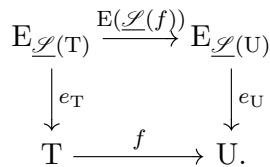
\includegraphics[keepaspectratio]{images/part001_16180f76.jpg}}
\end{enumerate}

对第一个图，这由 I, p. 54 的公式 (2) 得出；对第二个图，它是定义的直接推论。由此推出：对 B 上的每一对层 \((\mathcal{F},\mathcal{G})\) 与平展 B-空间的每一对 (T,U)，上面所考虑的映射 \(\varphi\mapsto\mathrm{E}(\varphi)\) 与 \(f\mapsto\underline{\mathcal{L}}(f)\) 都是双射。

这些结果使得我们能从关于 B 上的层的一个命题推出关于平展 B-空间的一个命题，反之亦然。

\subsection{层的直像与逆像}

设 A 与 B 为拓扑空间，\(u: A \rightarrow B\) 为连续映射。

设 \(\mathcal{F} = (\mathcal{F}(\mathrm{U}), f_{\mathrm{UV}})\) 为 A 上的一个预层。我们如下定义 B 上的一个预层 \(\mathcal{F}'\)：对 B 的每个开集 U，令 \(\mathcal{F}'(\mathrm{U}) = \mathcal{F}(u^{-1}(\mathrm{U}))\)；对 B 的每对开集 (U, V) （满足 U \(\subset\) V 者），令 \(f_{\mathrm{UV}}' = f_{u^{-1}(\mathrm{U})u^{-1}(\mathrm{V})}\)。于是 \((\mathcal{F}'(\mathrm{U}), f_{\mathrm{UV}}')\) 是 B 上的一个预层。我们把它记作 \(u_{*}(\mathcal{F})\)，并称之为预层 \(\mathcal{F}\) 在映射 u 下的直像预层。

若 \((\mathrm{U}_{i})_{i\in\mathrm{I}}\) 是 B 的一族开集，则有 \(u^{-1}(\bigcup_{i\in\mathrm{I}}\mathrm{U}_{i})=\bigcup_{i\in\mathrm{I}}u^{-1}(\mathrm{U}_{i})\) 与 \(u^{-1}(\bigcap_{i\in\mathrm{I}}\mathrm{U}_{i})=\bigcap_{i\in\mathrm{I}}u^{-1}(\mathrm{U}_{i})\) （E, II, p. 25, prop. 3 与 4）。由此立即得出：若 F 具有层的性质 \((\mathrm{F}_{1})\)（相应地 \((\mathrm{F}_{2})\)）(I, p. 43)，则 \(u_{*}(\mathcal{F})\) 亦然。因此，一个层的直像是层。

设 \(\mathcal{F}_1\) 与 \(\mathcal{F}_2\) 为 A 上的预层，\(\varphi\colon\mathcal{F}_1\to\mathcal{F}_2\) 为预层的一个态射。于是存在唯一的预层态射 \(u_*\varphi\colon u_*\mathcal{F}_1\to u_*\mathcal{F}_2\)，使得对 B 的每个开集 U，映射 \((u_*\varphi)(U)\colon(u_*\mathcal{F}_1)(U)\to(u_*\mathcal{F}_2)(U)\) 就是映射 \(\varphi(u^{-1}(U))\colon\mathcal{F}_{1}(u^{-1}(U))\to\mathcal{F}_{2}(u^{-1}(U)).\) 若 \(\mathcal{F}_{3}\) 是 A 上的预层且 \(\psi\colon\mathcal{F}_{2}\to\mathcal{F}_{3}\) 是预层的态射，则有 \(u_{*}(\psi\circ\varphi)=u_{*}(\psi)\circ u_{*}(\varphi)\)。

设 C 为拓扑空间，\(v: B \to C\) 为连续映射。若 \(\mathcal{F}\) 是 A 上的预层，则预层 \(v_{*}(u_{*}(\mathcal{F}))\) 与 \((v \circ u)_{*}(\mathcal{F})\) 相同。若 \(\varphi: \mathcal{F}_{1} \to \mathcal{F}_{2}\) 是 A 上的预层态射，则有等式 \(v_{*}(u_{*}(\varphi)) = (v \circ u)_{*}(\varphi)\)。

例 1. --- 设 B 为拓扑空间，A 为 B 的一个子空间，\(\mathcal{F} = (\mathcal{F}(U), f_{\mathrm{UV}})\) 为 A 上的一个预层。用 \(i: A \to B\) 表示典范单射。于是有 \(i_*(\mathcal{F}) = (\mathcal{F}'(U), f_{\mathrm{UV}}')\)，其中对 B 的每个开集 U 有 \(\mathcal{F}'(U) = \mathcal{F}(U \cap A)\)，而对 B 的每对开集 (U, V) （满足 \(U \subset V\) 者）有 \(f_{\mathrm{UV}}' = f_{(\mathrm{U} \cap A)(\mathrm{V} \cap A)}\)。

现在设 \(\mathcal{G}\) 为 B 上的一个预层。我们定义预层 \(\mathcal{G}\) 在 \(u\) 下的逆像，并用 \(u^{*}(\mathcal{G})\) 表示层 \(\underline{\mathcal{C}}_{\mathrm{B}}(\mathrm{A};\mathrm{E}_{\mathcal{G}})\) （A 上的、以 B-空间 \(\mathrm{E}_{\mathcal{G}}\) 为值的 B-态射所成的层）（I, p. 45, 例 4）。它典范同构于 A-平展空间 \(\mathrm{A} \times_{\mathrm{B}} \mathrm{E}_{\mathcal{G}}\) 的截面在 A 上所成的层 (I, p. 9, prop. 3)。由此我们推出 (I, p. 52, 例 2) 一个典范同构 \(\varphi\)，它把与 \(u^{*}(\mathcal{G})\) 相伴的平展空间映到 A-空间 \(\mathrm{A} \times_{\mathrm{B}} \mathrm{E}_{\mathcal{G}}\) 上。此外，若 \(\mathcal{G}\) 是层，则对 A 的每一点 \(a\) 有一个典范双射 \(\psi_{a}: u^{*}(\mathcal{G})_{a} \to \mathcal{G}_{u(a)}\)：对 \(a\) 在 A 中的每个开邻域 U 与每个 B-态射 \(f: \mathrm{U} \to \mathrm{E}_{\mathcal{G}}\)，我们有

\[
\varphi ([ \mathrm{U}, f, a ]) = (a, f (a)), \quad \psi_ {a} ([ \mathrm{U}, f, a ]) = f (a).
\]

设 \(\mathcal{G}_1\) 与 \(\mathcal{G}_2\) 为 B 上的预层，\(\varphi\colon\mathcal{G}_1\to\mathcal{G}_2\) 为预层的一个态射。由 B-平展空间的态射 \(\mathrm{E}(\varphi)\colon\mathrm{E}_{\mathcal{G}_1}\to\mathrm{E}_{\mathcal{G}_2}\) 经基变换，我们导出 A-平展空间的一个态射 \(\mathrm{A}\times_{\mathrm{B}}\mathrm{E}_{\mathcal{G}_1}\to\mathrm{A}\times_{\mathrm{B}}\mathrm{E}_{\mathcal{G}_2}\)，从而导出 A 上的层的一个态射 \(u^{*}(\varphi)\colon u^{*}(\mathcal{G}_{1})\to u^{*}(\mathcal{G}_{2})\)。设 \(\mathcal{G}_3\) 为 B 上的预层，\(\psi\colon\mathcal{G}_2\to\mathcal{G}_3\) 为预层的一个态射。于是有等式 \(u^{*}(\psi\circ\varphi)=u^{*}(\psi)\circ u^{*}(\varphi)\)。

设 C 为拓扑空间，\(v\colon B \to C\) 为连续映射。若 \(\mathcal{G}\) 是 C 上的预层，则层 \(u^{*}(v^{*}(\mathcal{G}))\) 与 \((v \circ u)^{*}(\mathcal{G})\) 典范地等同 (I, p. 5)。若 \(\varphi\colon\mathcal{G}_{1} \to \mathcal{G}_{2}\) 是 C 上的预层态射，则更有 \(u^{*}(v^{*}(\varphi)) = (v \circ u)^{*}(\varphi)\)。

注. --- I, p. 53 中的典范态射 \(\sigma_{\mathcal{G}}\colon\mathcal{G}\to\widetilde{\mathcal{G}}\) 用平展空间的语言对应于 I, p. 53 命题 2 的同构 \(j_{\mathcal{G}}\)。由此推出 \(u^{*}(\sigma_{\mathcal{G}})\) 是同构。特别地，若 \(A = B\) 且 \(u = \mathrm{Id}_A\)，则预层 \(u^{*}(\mathcal{F})\) 就是层 \(\widetilde{\mathcal{F}}\)。

例 2. --- 设 B 为拓扑空间，A 为 B 的一个子空间。用 \(i\colon\mathrm{A}\to\mathrm{B}\) 表示典范单射。对 B 上的每个层 \(\mathcal{G}\)，用 \(\mathcal{G}_{\mathrm{A}}\) 表示层 \(i^{*}(\mathcal{G})\)，并称 \(\mathcal{G}_{\mathrm{A}}\) 为由层 \(\mathcal{G}\) 在 A 上诱导的层。层 \(\mathcal{G}_{\mathrm{A}}\) 等同于层 \(\underline{\mathcal{L}}(\mathrm{A};(\mathrm{E}_{\mathcal{G}})_{\mathrm{A}})\) ，即由 \(\mathrm{E}_{\mathcal{G}}\) 在 A 上诱导的 A-平展空间的截面所成的层。

设 A 是 B 的一个开子空间，\(\mathcal{G}\) 是 B 上的一个层。按定义，层 \(\mathcal{G}_{\mathrm{A}}\) 是层 \(\widetilde{\mathcal{G}}\mid \mathrm{A}\) （由 \(\widetilde{\mathcal{G}}\) 限制到开集 A 而得者）(I, p. 43)。设 \(\sigma_{\mathcal{G}}\colon \mathcal{G}\to \widetilde{\mathcal{G}}\) 为典范同构 (I, p. 55, cor. 1)。于是 \(\sigma_{\mathcal{G}}\mid \mathrm{A}\) 是从层 \(\mathcal{G}\mid \mathrm{A}\) 到层 \(\mathcal{G}_{\mathrm{A}}\) 上的一个典范同构，称为从 \(\mathcal{G}\mid \mathrm{A}\) 到 \(\mathcal{G}_{\mathrm{A}}\) 上的典范同构。

\subsection{\texorpdfstring{同态 \(\alpha\) 与 \(\beta\)；伴随}{同态 alpha 与 beta；伴随}}

设 A 与 B 为拓扑空间，\(u\colon\mathrm{A}\to\mathrm{B}\) 为连续映射。设 \(\mathcal{G}\) 为 B 上的一个预层。由预层直像的定义，层 \(u_{*}u^{*}\mathcal{G}\) 在 B 的开集 U 上的截面是层 \(u^{*}\mathcal{G}\) 在 A 的开集 \(u^{-1}(\mathrm{U})\) 上的截面，也就是一个 B-态射 \(u^{-1}(\mathrm{U})\to\mathrm{E}_{\mathcal{G}}\)。于是，下述对应定义了一个层的态射 \(\widetilde{\mathcal{G}}\to u_{*}u^{*}\mathcal{G}\)：把截面 \(s\) （\(\mathrm{E}_{\mathcal{G}}\) 在 B 的一个开集 U 上的）对应为截面 \(s\circ u\) （\(\mathrm{E}_{\mathcal{G}}\) 在 \(u^{-1}(\mathrm{U})\) 上的）。该态射与典范态射 \(\sigma_{\mathcal{G}}\colon\mathcal{G}\to\widetilde{\mathcal{G}}\) （I, p. 53）的复合是一个预层态射 \(\mathcal{G}\to u_{*}u^{*}\mathcal{G}\)，将记作 \(\beta_{\mathcal{G}}^{u}\)，甚至记作 \(\beta_{\mathcal{G}}\) （当映射 \(u\) 无歧义时）。

注. --- 1) 设 A、B、C 为拓扑空间，\(u\colon A \to B\)、\(v\colon B \to C\) 为连续映射；令 \(w = v \circ u\)。设 \(\mathcal{G}\) 为 C 上的一个预层。

设 U 为 C 的开集，s 为 \(E_{G}\) 在 U 上的一个截面。于是 \(\beta_{\mathcal{G}}^{v}(s)\) 是截面 \(s \circ v\) （\(E_{G}\) 在 \(v^{-1}(U)\) 上的），而 \(v_{*}(\beta_{v^{*}\mathcal{G}}^{u})(\beta_{\mathcal{G}}^{v}(s))\) 是截面 \(s \circ v \circ u = s \circ w\) （\(E_{G}\) 在 \(u^{-1}(v^{-1}(U)) = w^{-1}(U)\) 上的）。

由此得 \(\beta_{\mathcal{G}}^{w} = v_{*}(\beta_{v^{*}\mathcal{G}}^{u})\circ \beta_{\mathcal{G}}^{v}\)。

\begin{enumerate}
\def\labelenumi{\arabic{enumi})}
\setcounter{enumi}{1}
\tightlist
\item
  若 \(\gamma\colon\mathcal{G}_{1}\to\mathcal{G}_{2}\) 是 B 上的预层态射，则预层态射 \(\beta_{\mathcal{G}_{2}}\circ\gamma\) 与 \(u_{*}u^{*}(\gamma)\circ\beta_{\mathcal{G}_{1}}\) 相等。事实上，若 V 是 B 的开集且 \(s\in\mathcal{G}_{1}(V)\)，则 \(\beta_{\mathcal{G}_{1}}(s)\) 是截面 \(t\) （A \(\times_{B}E_{\mathcal{G}_{1}}\) 在 \(u^{-1}(V)\) 上的），由 \(x\mapsto(x,[V,s,u(x)])\) 定义。于是 \(t\) 在 \(u^{*}(\gamma)\) 下的像是 A \(\times_{B}E_{\mathcal{G}_{2}}\) 在 \(u^{-1}(V)\) 上由 \(x\mapsto(x,[V,\gamma(s),u(x)])\) 给出的截面。由此得 \(u_{*}u^{*}(\gamma)\circ\beta_{\mathcal{G}_{1}}(s)=\beta_{\mathcal{G}_{2}}(\gamma(s))\)。
\end{enumerate}

命题 4. --- 设 A 与 B 为拓扑空间，\(u\colon A\to B\) 为连续映射，\(\mathcal{G}\) 为 B 上的一个预层，\(\mathcal{F}\) 为 A 上的一个层。

对每个预层态射 \(\varphi\colon\mathcal{G}\to u_{*}\mathcal{F}\)，存在唯一的层的态射 \(\psi\colon u^{*}(\mathcal{G})\to\mathcal{F}\) 满足 \(\varphi=u_{*}(\psi)\circ\beta_{\mathcal{G}}\)。

换言之，典范映射

\[
\operatorname{Mor} \left(u ^ {*} (\mathcal {G}), \mathcal {F}\right)\rightarrow \operatorname{Mor} \left(\mathcal {G}, u _ {*} (\mathcal {F})\right), \quad \psi \mapsto u _ {*} (\psi) \circ \beta_ {\mathcal {G}}
\]

是双射。

采用命题 4 的记号，我们有时记 \(\psi = \varphi^{\sharp}\) 与 \(\varphi = \psi^{\flat}\)。

我们来证明命题 4。把注 2 应用于态射 \(\sigma_{\mathcal{G}}: \mathcal{G} \to \widetilde{\mathcal{G}}\)，便知态射 \(\beta_{\mathcal{G}}\) 等于复合

\[
u _ {*} (u ^ {*} (\sigma_ {\mathcal {G}}) ^ {- 1}) \circ \beta_ {\widetilde {\mathcal {G}}} \circ \sigma_ {\mathcal {G}},
\]

其中 \(u^{*}(\sigma_{\mathcal{G}}) \colon u^{*}(\mathcal{G}) \to u^{*}(\widetilde{\mathcal{G}})\) 是 I, p. 58 的注中的典范同构。设 \(\widetilde{\varphi} \colon \widetilde{\mathcal{G}} \to u_{*}\mathcal{F}\) 为唯一的层的态射，满足 \(\widetilde{\varphi} \circ \sigma_{\mathcal{G}} = \varphi\) (I, p. 54, prop. 3)。于是只需证明：存在唯一的层的态射 \(\widetilde{\psi} \colon u^{*}(\mathcal{G}) \to \mathcal{F}\) 满足 \(u_{*}(\widetilde{\psi}) \circ \beta_{\widetilde{\mathcal{G}}} = \widetilde{\varphi}\)。

因此我们可以假设 \(\mathcal{G}\) 是层。为使层的态射 \(\psi: u^{*}(\mathcal{G}) \to \mathcal{F}\) 满足命题 4 的结论，必须且只需：对 B 的每个开集 V 与每个截面 \(t\) （\(\mathrm{E}_{\mathcal{G}}\) 在 V 上的），有

\[
\varphi_{\mathrm{V}}(t) = \psi_{u^{-1}(\mathrm{V})}(t \circ u \mid u^{-1}(\mathrm{V})).\tag{6}
\]

设 \(U_{0}\) 为 A 的一个开子集，\(s_{0}\) 为 \(u^{*}(\mathcal{G})(\mathrm{U}_{0})\) 的一个元素，换言之，是从 \(U_{0}\) 到 \(E_{\mathcal{G}}\) 中的一个 B-态射。设 \(\mathrm{S}(\mathrm{U}_{0}, s_{0})\) 为三元组 \((\mathrm{U}, \mathrm{V}, t)\) 所成的集，其中 U 是 A 的含于 \(U_{0}\) 的开子集，V 是 B 的满足 \(u(\mathrm{U}) \subset \mathrm{V}\) 的开子集，而 t 是 \(E_{\mathcal{G}}\) 在 V 上的一个截面，且满足

\[
t \circ u \mid \mathrm{U} = s _ {0} \mid \mathrm{U}.\tag{7}
\]

若 \(U_{1}\) 与 \(U_{2}\) 是 A 的开子集且 \(U_{1} \subset U_{2}\)，则用 \(f_{U_{1}U_{2}}\) 表示限制映射 \(\mathcal{F}(U_{2}) \to \mathcal{F}(U_{1})\)。于是对每个 \((\mathrm{U}, \mathrm{V}, t) \in \mathrm{S}(\mathrm{U}_{0}, s_{0})\)，我们有关系式

\[
\begin{array}{l} f_{\mathrm{U}\mathrm{U}_{0}}(\psi_{\mathrm{U}_{0}}(s_{0})) = \psi_{\mathrm{U}}(s_{0} \mid \mathrm{U}) \\ \qquad = \psi_{\mathrm{U}}(t \circ u \mid \mathrm{U}) \\ \qquad = f_{\mathrm{U}u^{-1}(\mathrm{V})}(\psi_{u^{-1}(\mathrm{V})}(t \circ u \mid u^{-1}(\mathrm{V}))). \end{array}
\]

因此，若 \(\psi \colon u^{*}(\mathcal{G})\to \mathcal{F}\) 满足 (6)，则我们有

\[
f_{\mathrm{U}\mathrm{U}_{0}}(\psi_{\mathrm{U}_{0}}(s_{0})) = f_{\mathrm{U}u^{-1}(\mathrm{V})}(\varphi_{\mathrm{V}}(t)).\tag{8}
\]

我们来证明：对每一点 \(a\) （属于 \(\mathrm{U}_0\) 者），存在三元组 \((\mathrm{U},\mathrm{V},t)\in \mathrm{S}(\mathrm{U}_0,s_0)\) 使得 \(a\in \mathrm{U}\)。事实上，设 \(a\) 为 \(\mathrm{U}_0\) 的一点。存在 B 中包含 \(u(a)\) 的开邻域 V，以及截面 \(t\) （平展空间 \(\mathbf{E}_{\mathcal{G}}\) 在 V 上的），使得 \(t(u(a)) = s_0(a)\) (I, p. 33, prop. 9)。令 \(\mathrm{U}_1 = u^{-1} (\mathrm{V})\cap \mathrm{U}_0\)。截面 \(s_0\mid \mathrm{U}_1\) 与 \(t\circ u\mid \mathrm{U}_1\) ——即 \(\mathrm{U}_1\) 上的平展空间 \(\mathbf{E}_{\mathcal{G}}\times_{\mathrm{B}}\mathrm{U}_1\) 的截面——在点 \(a\) 处相合。由 I, p. 34 的 prop. 11, b)，二者相合的点所成的集是 \(\mathrm{U}_1\) 的一个包含 \(a\) 的开集 U。于是三元组 \((\mathrm{U},\mathrm{V},t)\) 属于 \(\mathrm{S}(\mathrm{U}_0,s_0)\)。

于是，公式 (8) 与层的性质 \((\mathrm{F}_{1})\) (I, p. 43) 蕴涵 \(\psi\) 的唯一性。

设 (U, V, t) 与 \((\mathrm{U}^{\prime}, \mathrm{V}^{\prime}, t^{\prime})\) 为 \(\mathrm{S}(\mathrm{U}_{0}, s_{0})\) 的元素。由关系式 (7)，t 与 \(t^{\prime}\) 在 \(u(\mathrm{U} \cap \mathrm{U}^{\prime})\) 上的限制相合。由 I, p. 34 的 prop. 11, b)，存在 B 的开集 W 满足 \(u(\mathrm{U} \cap \mathrm{U}^{\prime}) \subset \mathrm{W} \subset \mathrm{V} \cap \mathrm{V}^{\prime}\) 且 \(t \mid W = t^{\prime} \mid W\)。因此我们有

\[
f_{u^{-1}(\mathrm{W})u^{-1}(\mathrm{V})}(\varphi_{\mathrm{V}}(t)) = \varphi_{\mathrm{W}}(t\mid \mathrm{W}) = \varphi_{\mathrm{W}}(t^{\prime}\mid \mathrm{W}) = f_{u^{-1}(\mathrm{W})u^{-1}(\mathrm{V}^{\prime})}(\varphi_{\mathrm{V}^{\prime}}(t^{\prime}))
\]

从而

\[
f_{(\mathrm{U}\cap\mathrm{U}^{\prime})u^{-1}(\mathrm{V})}(\varphi_{\mathrm{V}}(t)) = f_{(\mathrm{U}\cap\mathrm{U}^{\prime})u^{-1}(\mathrm{V}^{\prime})}(\varphi_{\mathrm{V}^{\prime}}(t^{\prime})).\tag{9}
\]

由层 F 的性质 \((\mathrm{F}_{1})\) 与 \((\mathrm{F}_{2})\)，存在唯一的元素 \(s'\) （\(\mathcal{F}(\mathrm{U}_{0})\) 的），使得对每个三元组 \((\mathrm{U},\mathrm{V},t)\) （取自

\(\mathrm{S}(\mathrm{U}_{0},s_{0})\) 者），有：

\[
f_{\mathrm{U}\mathrm{U}_{0}}(s^{\prime}) = f_{\mathrm{U}u^{-1}(\mathrm{V})}(\varphi_{\mathrm{V}}(t)).\tag{10}
\]

把这个元素记作 \(\psi_{\mathrm{U}_{0}}(s_{0})\)。

设 \(U_{1}\) 为含于 \(U_{0}\) 的开集，且 \(s_{1}=s_{0}|U_{1}\)。若 \((\mathrm{U},\mathrm{V},t)\in\mathrm{S}(\mathrm{U}_{1},s_{1})\)，则 U 是含于 \(U_{0}\) 的开集且 \(t\circ u|U=s_{1}|U=s_{0}|U\)，因此 \((\mathrm{U},\mathrm{V},t)\in\mathrm{S}(\mathrm{U}_{0},s_{0})\)，而关系式 (10) 这时蕴涵

\[
f_{\mathrm{U}\mathrm{U}_{1}}(f_{\mathrm{U}_{1}\mathrm{U}_{0}}(\psi_{\mathrm{U}_{0}}(s_{0}))) = f_{\mathrm{U}\mathrm{U}_{0}}(\psi_{\mathrm{U}_{0}}(s_{0})) = f_{\mathrm{U}u^{-1}(\mathrm{V})}(\varphi_{\mathrm{V}}(t)).
\]

由 \(\psi_{\mathrm{U}_{1}}(s_{1})\) 的定义，我们于是有 \(\psi_{\mathrm{U}_{1}}(s_{1}) = f_{\mathrm{U}_{1}\mathrm{U}_{0}}(\psi_{\mathrm{U}_{0}}(s_{0}))\)。这就证明了族 \(\psi = (\psi_{\mathrm{U}})\) 是从 \(u^{*}(\mathcal{G})\) 到 \(\mathcal{F}\) 中的层的态射。

我们来证明 \(\psi\) 满足关系式 (6)。设 V 为 B 的开子集，\(t\) 为 \(\mathrm{E}_{\mathcal{G}}\) 在 V 上的一个截面。若 \(\mathrm{U} = u^{-1}(\mathrm{V})\) 且 \(s = t \circ u \mid \mathrm{U}\)，则三元组 \((\mathrm{U}, \mathrm{V}, t)\) 属于 \(\mathrm{S}(\mathrm{U}, s)\)，而关系式 (6) 是关系式 (10) （应用到 \(\mathrm{U} = \mathrm{U}_0\)）的直接推论。

命题 5. — 设 A 与 B 为拓扑空间，u: A → B 为连续映射。

\begin{enumerate}
\def\labelenumi{\alph{enumi})}
\tightlist
\item
  设 \(\mathcal{G}_1\) 与 \(\mathcal{G}_2\) 为 B 上的预层，\(\gamma\colon\mathcal{G}_1\to\mathcal{G}_2\) 为预层的一个态射。再设 \(\mathcal{F}\) 为 A 上的层，\(\varphi\colon\mathcal{G}_2\to u_*\mathcal{F}\) 为预层的一个态射。我们有等式
\end{enumerate}

\[
(\varphi \circ \gamma) ^ {\sharp} = \varphi^ {\sharp} \circ u ^ {*} (\gamma).\tag{11}
\]

\begin{enumerate}
\def\labelenumi{\alph{enumi})}
\setcounter{enumi}{1}
\tightlist
\item
  设 \(\mathcal{F}_1\) 与 \(\mathcal{F}_2\) 为 A 上的层，\(\mathcal{G}\) 为 B 上的一个预层。设 \(\varphi\colon\mathcal{F}_1\to\mathcal{F}_2\) 为层的一个态射，\(\gamma\colon\mathcal{G}\to u_*\mathcal{F}_1\) 为预层的一个态射。我们有关系式
\end{enumerate}

\[
(u _ {*} (\varphi) \circ \gamma) ^ {\sharp} = \varphi \circ \gamma^ {\sharp}.
\]

\begin{enumerate}
\def\labelenumi{\alph{enumi})}
\tightlist
\item
  由 \(\varphi^{\sharp}\) 的定义与 I, p. 60 的注 2，我们有
\end{enumerate}

\[
\varphi \circ \gamma = u _ {*} (\varphi^ {\sharp}) \circ \beta_ {\mathcal {G} _ {2}} \circ \gamma = u _ {*} (\varphi^ {\sharp}) \circ u _ {*} u ^ {*} (\gamma) \circ \beta_ {\mathcal {G} _ {1}}.
\]

因此，\(\varphi \circ \gamma = u_{*}(\varphi^{\sharp}\circ u^{*}(\gamma))\circ \beta_{\mathcal{G}_{1}}\)；由此得关系式 (11)。

\begin{enumerate}
\def\labelenumi{\alph{enumi})}
\setcounter{enumi}{1}
\tightlist
\item
  由 \(\gamma^{\sharp}\) 的定义，我们有
\end{enumerate}

\[
u _ {*} (\varphi) \circ \gamma = u _ {*} (\varphi) \circ u _ {*} (\gamma^ {\sharp}) \circ \beta_ {\mathcal {G}} = u _ {*} (\varphi \circ \gamma^ {\sharp}) \circ \beta_ {\mathcal {G}},
\]

从而得到所宣布的关系式，这里用到了 \((u_{*}(\varphi)\circ\gamma)^{\sharp}\) 的定义。

令 \(\alpha_{\mathcal{F}} = \mathrm{Id}_{u_*(\mathcal{F})}^\sharp\)；它是唯一的层的态射 \(\rho \colon u^*(u_*(\mathcal{F})) \to \mathcal{F}\)，满足

\[
\operatorname{Id} _ {u _ {*} (\mathcal {F})} = u _ {*} (\rho) \circ \beta_ {u _ {*} (\mathcal {F})}.
\]

把关系式 (11) 应用于 \(\mathcal{G}_2 = u_*(\mathcal{F})\) 与态射 \(\varphi = \mathrm{Id}_{u_*(\mathcal{F})}\)，就对每个预层态射 \(\gamma\colon\mathcal{G}\to u_*(\mathcal{F})\) 给出分解式

\[
\gamma^ {\sharp} = \alpha_ {\mathcal {F}} \circ u ^ {*} (\gamma).
\]

于是由命题 4 推出：对每个层的态射 \(\psi\) （从 \(u^{*}(\mathcal{G})\) 到 \(\mathcal{F}\) 中的），\(\psi^{\flat}\) 是唯一的态射 \(\varphi\colon\mathcal{G}\to u_{*}(\mathcal{F})\) 满足 \(\psi=\alpha_{\mathcal{F}}\circ u^{*}(\varphi)\)。

例. --- 1) 考察拓扑空间 B、B 的子空间 A，并用 \(i\colon A \to B\) 表示典范单射。设 \((E,p)\) 与 \((E',p')\) 为 B-空间。取 \(\mathcal{G}\) 为层 \(\underline{\mathcal{M}or}_{B}(E;E')\) （I, p. 45, 例 4），取 \(\mathcal{F}\) 为层 \(\underline{\mathcal{M}or}_{A}(E_{A};E_{A}')\)。对 B 的每个开集 V 与每个 V-态射 \(f\colon E_{V} \to E_{V}'\)，令 \(\varphi_{V}(f) = f_{V \cap A}\)，其中 \(f_{V \cap A}\) 是 \((V \cap A)\) -态射 （从 \(E_{V \cap A}\) 到 \(E_{V \cap A}'\) 中的、由 \(f\) 诱导者）。如此定义的族 \(\varphi = (\varphi_{V})\) 是从 \(\mathcal{G}\) 到 \(i_*\mathcal{F}\) 中的层的态射。由命题 4，存在唯一的层的态射 \(\psi\colon \underline{\mathcal{M}or}_{B}(E;E')_{A} \to \underline{\mathcal{M}or}_{A}(E_{A};E_{A}')\)，使得有

\[
\psi_ {\mathrm{V} \cap \mathrm{A}} (\sigma_ {\mathcal {G}} (\mathrm{V}, f) \mid \mathrm{V} \cap \mathrm{A}) = f _ {\mathrm{V} \cap \mathrm{A}}\tag{12}
\]

对 B 的每个开集 V 与每个 \(f \in \mathcal{C}_{\mathrm{V}}(\mathrm{E}_{\mathrm{V}}; \mathrm{E}_{\mathrm{V}}^{\prime})\) 成立。态射 \(\psi\) 称为从 \(\underline{\mathcal{M}or_{B}}(\mathrm{E}; \mathrm{E}^{\prime})_{\mathrm{A}}\) 到 \(\underline{\mathcal{M}or_{A}}(\mathrm{E}_{\mathrm{A}}; \mathrm{E}_{\mathrm{A}}^{\prime})\) 中的典范态射。

若 A 缩为一个单点 \(a\)，则该态射等同于从 \(a\) 处的茎（层 \(\underline{\mathcal{M}or}_{\mathrm{B}}(\mathrm{E};\mathrm{E}^{\prime})\) 的）到集合 \(\mathcal{C}(\mathrm{E}_a;\mathrm{E}_a')\) 中的态射。

通过过渡到子层，态射 \(\psi\) 诱导出从 \(\mathcal{I}som_{\mathrm{B}}(\mathrm{E};\mathrm{E}')_{\mathrm{A}}\) 到 \(\mathcal{I}som_{\mathrm{A}}(\mathrm{E}_{\mathrm{A}};\mathrm{E}_{\mathrm{A}}^{\prime})\) 中的一个典范态射。

\begin{enumerate}
\def\labelenumi{\arabic{enumi})}
\setcounter{enumi}{1}
\tightlist
\item
  设 A、B、C 为拓扑空间，\(u\colon A\to B\)、\(v\colon B\to C\) 为连续映射；令 \(w=v\circ u\)。设 E 与 E' 为 C-空间。从 \(\underline{\mathcal{M}or}_{C}(E;E')_{A}\) 到 \(\underline{\mathcal{M}or}_{A}(E_{A};E'_{A})\) 中的典范态射是这样一个态射与另一个典范态射的复合：前者为 \(\underline{\mathcal{M}or}_{C}(E;E')_{A}\to\underline{\mathcal{M}or}_{B}(E_{B};E'_{B})_{A}\) （由 \(\underline{\mathcal{M}or}_{C}(E;E')_{B}\) 到 \(\underline{\mathcal{M}or}_{B}(E_{B};E'_{B})\) 中的典范态射导出者），后者为从 \(\underline{\mathcal{M}or}_{B}(E_{B},E'_{B})_{A}\) 到 \(\underline{\mathcal{M}or}_{A}(E_{A},E'_{A})\) 中的典范态射。
\end{enumerate}
